\pagestyle{scrheadings}
\ihead[]{\rightmark}
\ohead[]{Iván Rodríguez Méndez}
\ofoot[]{\thepage{}}
\chapter{Experimentación y discusión}\label{ch:capitulo5}
\section{Equipos de trabajo y sistemas}
En esta sección especificaremos los equipos con los que hemos trabajado para realizar las simulaciones y los experimentos de los que hablaremos en este capítulo.

Para la realización de los experimentos hemos trabajado principalmente con dos equipos, uno haciendo de cliente y el otro de servidor.
Las características de los equipos son las siguientes:
\begin{itemize}
\item \textbf{EQUIPO 1 (SERVIDOR)}:
\begin{itemize}
\item \textbf{Procesador}: 4x Intel(R) Core(TM) i7-3517U CPU @ 1.90 Ghz
\item \textbf{Memoria RAM}: 8 Gb
\item \textbf{Disco duro}: SSD
\item \textbf{Tarjeta Gráfica}: Nvidia GeForce GT 635M 2 Gb
\item \textbf{Sistema operativo}: Ubuntu 16.04 LTS 64 bits Kernel 4.4.0-22 generic
\end{itemize}
\item \textbf{EQUIPO 2 (CLIENTE)}:
\begin{itemize}
\item \textbf{Procesador}: 2x Intel(R) Core(TM)2 Duo CPU E7500 @ 2.93Ghz
\item \textbf{Memoria RAM}: 4 Gb
\item \textbf{Disco duro}: HDD
\item \textbf{Tarjeta Gráfica}: Tarjeta integrada Intel 256 MB
\item \textbf{Sistema operativo}: Kubuntu 16.04 LTS 64 bits Kernel 4.4.0-22 generic
\end{itemize}
\end{itemize}
El equipo que hace de cliente es el encargado de ejecutar todos los códigos en MATLAB para gestionar el correcto funcionamiento de la simulación y además almacena todos sus parámetros.
Por otra parte el equipo que hace de servidor es el encargado de ejecutar V-REP y por lo tanto de hacer todos los cálculos relacionados con el \textit{engine} de físicas (tipo \textit{bullet}).
Este motor es el que más recursos computacionales necesita y por eso es más adecuado usar un equipo con mejor procesador para ello.
% * <amorellg@ull.edu.es> 2016-06-06T17:47:36.598Z:
%
% > pre-visualización
%
% Seguro que es pre? Más bien visualización. Además, si luego dices que los experimentos los haces en modo headless, no tiene sentido decir que la razón de usar el más potente es por el 3D. Mejor poner que el engine físico (que no he visto aún si has dicho el que usaste, Bullet imagino) es el que más recursos computacionales necesita y por eso es más adecuado usar el equipo con mejor procesador para eso
%
% ^ <alu0100765755@ull.edu.es> 2016-06-06T23:55:35.368Z.
Hemos elegido que el equipo más potente sea el que ejecute V-REP ya que la representación 3D requiere bastante potencia de cómputo y el motor de físicas del \textit{engine} también, por otra parte gracias a los \textit{trigger} de sincronización el equipo más lento no tiene problemas para ejecutar el código ya que el servidor espera a que acabe cada ciclo de simulación.

También tenemos la posibilidad de ejecutar el sistema cliente-servidor en un solo equipo.
Para este tipo de simulaciones elegiremos el equipo 1 por ser el más potente de los dos.

\section{Estructura básica de los experimentos.}
% * <amorellg@ull.edu.es> 2016-06-06T17:50:00.877Z:
%
% > , escenas, modelos y código
%
% esto lo quitaría
%
% ^ <alu0100765755@ull.edu.es> 2016-06-06T23:58:02.798Z:
%
% Listo !
%
% ^ <alu0100765755@ull.edu.es> 2016-06-06T23:58:05.000Z.

Como comentamos en el capítulo \ref{ch:capitulo4}, realizaremos los experimentos usando el software V-REP conectado a MATLAB por medio de una API.
Hemos creado una serie de funciones (consultar apéndice \ref{ApendiceC}) para realizar la comunicación entre MATLAB y V-REP, y además algunas otras para modificar propiedades del simulador, nuestro modelo, etc .

Para la experimentación además hemos creado unos códigos de función principales que se encargarán de simular cada uno de los filtros estudiados en el capítulo \ref{ch:capitulo3}.
Estos códigos pueden ser consultados en el apéndice \ref{ApendiceC} en la séptima sección del mismo.

Para explicar el procedimiento seguido en los scripts de los experimentos sobre la localización del Pioneer P3-DX  lo mejor es enseñar el procedimiento a través de un algoritmo.
% * <amorellg@ull.edu.es> 2016-06-06T17:51:48.172Z:
%
% > nuestro Robot
%
% mejor "del Pioneer P3-DX"
%
% ^ <alu0100765755@ull.edu.es> 2016-06-06T23:59:41.184Z.
En total en la capítulo \ref{ch:capitulo3} estudiamos cuatro filtros diferentes por lo que tendríamos cuatro métodos con los que realizar pruebas y extraer diferentes datos, sin embargo la estructura organizativa de los scripts es la misma y por lo tanto aunque los códigos están diseñados para distintas herramientas el procedimiento seguido se ha mantenido en todos los experimentos.
% * <amorellg@ull.edu.es> 2016-06-06T17:53:14.187Z:
%
% > filtros
%
% métodos
%
% ^ <alu0100765755@ull.edu.es> 2016-06-07T00:00:28.889Z.

En el algoritmo \ref{alg:experimentos} podemos ver la estructura básica que presentan los códigos que implementan los experimentos en V-REP.
Antes de pasar a comentar algunas cuestiones acerca del algoritmo debemos saber que para que nuestro código sea funcional debemos tener creadas algunas escenas y modelos para poder cargarlos posteriormente desde MATLAB en V-REP.
En nuestro caso disponemos de 19 escenas diferentes ya que como explicaremos en la siguiente sección hay que testear el robot en diferentes situaciones para poder llegar a conclusiones lo más fehacientes posibles.
% * <amorellg@ull.edu.es> 2016-06-06T17:54:34.939Z:
%
% > fieles
%
% fehacientes
%
% ^ <alu0100765755@ull.edu.es> 2016-06-07T00:06:12.699Z.
Para lograr los diferentes coeficientes de rozamiento en nuestras escenas y por lo tanto los diferentes porcentajes de deslizamiento del robot lo que hemos hecho es utilizar el motor de físicas tipo \textit{bullet} (uno de los disponibles dentro de la simulación en V-REP) y hemos variado el tipo de física utilizada por el suelo, es decir, la fricción que presenta dicho material.
Para conseguir estos coeficientes de rozamiento lo que hemos realizado es una interpolación lineal del parámetro adimensional que controla dicha característica en el motor de físicas,  es decir, hemos visto cual es el caso de fricción baja y cual es el de fricción alta y hemos interpolado una serie de valores centrales.
Como resultado de esta interpolación hemos obtenido los distintos porcentajes de deslizamiento.
Por otro lado el diferencial de tiempo utilizado por este motor de físicas es de 50 $ms$  con lo que nos hemos asegurado de usar los mismos para nuestros scripts.
Las escenas disponibles para cargar desde nuestra API son las siguientes:
% * <amorellg@ull.edu.es> 2016-06-06T17:56:24.570Z:
%
% > escenas
%
% Pon antes de hablar de % de deslizamiento que hiciste una aproximación lineal del parámetro adimensional que tiene V-REP como entrada para el deslizamiento
%
% ^ <alu0100765755@ull.edu.es> 2016-06-07T00:14:39.450Z.
\begin{itemize}
\item \textbf{Escena con trayectoria recta:}En estas escenas colocamos todos los objetivos (conos) siguiendo una trayectoria recta y además disponemos de 11 balizas (cilindros) distribuidas de forma uniforme por el entorno.
Podemos ver la escena en la figura \ref{Escena-recta}.
Los porcentajes de deslizamiento para el robot disponibles en las escenas son los siguientes:
\begin{itemize}
\item Sin deslizamiento.
\item Deslizamiento del $3\%$.
\item Deslizamiento del $5\%$.
\item Deslizamiento del $7\%$.
\end{itemize}
\begin{figure}[ht!]
\centering
\includegraphics[scale=0.7]{V-REP-RECTA}
\caption{Escena trayectoria recta V-REP} \label{Escena-recta}
\end{figure}
Además para esta trayectoria también disponemos con variantes en las que modificamos el número de balizas, en concreto disponemos de una escena con tres balizas y otra con cinco.
\item \textbf{Escena con trayectoria cuadrada:} En estas escenas colocamos 4 objetivos formando un cuadrado y además disponemos de 9 balizas que también están distribuidas de forma uniforme por el entorno pero pueden reducirse según el experimento.
Podemos ver esta trayectoria en la figura \ref{Escena-cuadrado}.
Los porcentajes de deslizamiento disponibles para esta escena son:
\begin{itemize}
\item Sin deslizamiento.
\item Deslizamiento del $3\%$.
\item Deslizamiento del $5\%$.
\item Deslizamiento del $7\%$.
\end{itemize}
\begin{figure}[ht!]
\centering
\includegraphics[scale=0.7]{V-REP-CUADRADO}
\caption{Escena trayectoria cuadrada V-REP} \label{Escena-cuadrado}
\end{figure}
Al igual que para la recta, para esta escena también disponemos de unas modificaciones en la que variamos el número de balizas concretamente serán escenas con tres y cinco balizas. 
\item \textbf{Escena con trayectoria senoidal:} En estas escenas colocamos 7 objetivos para que el robot describa una trayectoria senoidal, además disponemos de 11 balizas en la escena aunque para algunos experimentos modificaremos el número de estas reduciendo el número a cinco y posteriormente a tres.
Podemos ver la trayectoria senoidal en la figura \ref{Escena-seno}.
Los porcentajes de deslizamiento son los mismos que para las dos escenas anteriores.
\begin{figure}[ht!]
\centering
\includegraphics[scale=0.7]{V-REP-SENO}
\caption{Escena trayectoria senoidal V-REP} \label{Escena-seno}
\end{figure}
\item \textbf{Trayectoria arbitraria:} En esta escena realizaremos un experimento final (que podemos ver en la figura \ref{Escena-circuito}) para determinar cual es el filtro que presenta el mejor comportamiento siguiendo una trayectoria con varias curvas, rectas y diferentes características que pongan en conjunto las de las tres escenas anteriores.
\begin{figure}[ht!]
\centering
\includegraphics[scale=0.7]{Circuito}
\caption{Escena trayectoria arbitraria V-REP} \label{Escena-circuito}
\end{figure}
\end{itemize}

% * <amorellg@ull.edu.es> 2016-06-06T18:07:20.765Z:
%
% > motor de físicas
%
% aquí al hablar del motor de física, pon el diferencial de tiempo con el que se han hecho los experimentos (ya vi que lo nombras más abajo, pero para que esté igualmente aquí que es donde dices cómo has configurado las escenas en V-REP)
%
% ^ <alu0100765755@ull.edu.es> 2016-06-07T00:21:37.429Z.
% * <amorellg@ull.edu.es> 2016-06-06T17:58:06.001Z:
%
% > deslizamiento
%
% aquí es donde podrías hablar de la aproximación que hiciste para poner el % de deslizamiento, y casi mejor mover este parrafillo arriba, antes de que digas que hay un % que aún no se sabe lo que representa
%
% ^ <alu0100765755@ull.edu.es> 2016-06-07T00:21:50.132Z.
Con la variedad de escenas conseguimos que las ruedas deslicen en mayor o menor medida y por lo tanto el robot sufra deslizamientos dentro de la escena.

Por otra parte disponemos de dos modelos del robot, uno que hará el papel de robot principal (figura \ref{Modelo_real}) y por lo tanto será el encargado de ejecutar los movimientos, y otro que será el robot estimado (figura \ref{Modelo_estimado}) y por lo tanto mostrará la estimación de la posición que Kalman ha realizado.
Los modelos utilizados como dijimos en el capítulo \ref{ch:capitulo4} serán los del \textbf{Pioneer P3-DX} ya que están pre-instalados en V-REP y su implementación es muy sencilla. 
Para la visualización de la trayectoria el robot real tiene implementado un marcador (una rotulador de un color específico) en su parte inferior, de esta manera podremos ver la trayectoria que ha seguido con mayor facilidad.
\begin{figure}[ht!]
\centering
\includegraphics[scale=0.7]{V-REP-REAL}
\caption{Modelo del robot real en V-REP} \label{Modelo_real}
\end{figure}

\begin{figure}[ht!]
\centering
\includegraphics[scale=0.7]{V-REP-ESTIMADO}
\caption{Modelo del robot estimado en V-REP} \label{Modelo_estimado}
\end{figure}

Una vez ya hemos hecho la introducción los modelos y las escenas implementadas podemos pasar a comentar el algoritmo seguido en la implementación de los experimentos (algoritmo \ref{alg:experimentos}).
En primer lugar, debemos introducir tres parámetros como entrada a las funciones experimentales.
Estos parámetros son, la escena seleccionada para ejecutar la simulación, el modelo de medida que usará el robot en sus sensores y por último la afectación de ruido en los sensores.
Con respecto al modelo de medida debemos añadir que esto es así ya que hemos implementado la posibilidad de tomar medidas de distancia usando el telémetro y por otra parte para añadir otras funciones de medida hemos configurado la posibilidad de medir diferencias angulares con respecto a los objetos de la escena tal y como se hace en la toolbox original \cite{toolbox_simo}.
Aunque el segundo modelo de medida no tenga una aplicación tan realista nos sirve para utilizar un modelo no lineal como parámetro en los filtros y así estudiar el comportamiento de estos.
Las expresiones de los modelos de medida son las siguientes:
\begin{itemize}
\item \textbf{Modelo de medida de distancia:}
\begin{equation}
Distancia = \sqrt[]{(x_{Robot}-x_{baliza})^{2}+(y_{Robot}-y_{baliza})^{2}}
\end{equation}\label{Modelo_distancia}
\item \textbf{Modelo de medida de ángulos:}
\begin{equation} \label{Modelo_angulo}
Angulo = \arctan{\frac{y_{Robot}-y_{Baliza}}{x_{Robot}-x_{Baliza}}}
\end{equation}
\end{itemize}
Para estos dos modelos también hemos implementado sus derivadas ya que algunos filtros lo requieren como parámetro de entrada, por ejemplo el \ac{EKF}.

Por otra parte en el algoritmo \ref{alg:experimentos} usaremos una estructura de datos para guardar todos los datos relacionados con el robot y así poder analizarlos posteriormente, estos datos son los siguientes:
\begin{itemize}
\item $pose_{actual}$
\item $Pose_{anterior}$
\item Dimensiones del robot.
\item Client ID.
\item Handles del robot.
\item Odometría.
\item Últimas rotaciones de las ruedas.
\item Medidas tomadas.
\item Trayectoria real.
\item Trayectoria estimada.
\item Ruido del robot.
\end{itemize}
\begin{algorithm}
\begin{algorithmic} [1]
\STATE{Cargamos el objeto de la API remota de V-REP}
\STATE{Seleccionamos la escena que queremos cargar}
\STATE{Nos conectamos a la IP deseada (local o de un equipo remoto)}
\STATE{Abrimos la conexión con V-REP}
\STATE{Enviamos mensajes de verificación, cargamos la escena y los modelos}
\STATE{Definimos la posición de los objetos dentro de la escena y las guardamos en un vector }
\STATE{Establecemos la configuración del robot: Velocidad lineal y angular máximas, distancia de medida del telémetro, etc}
\STATE{Seleccionamos el modo de medida solicitado (medida de distancia o de diferencia angular)}
\STATE{Leemos la posición de las balizas y los objetivos dentro de la escena, guardamos esta información en matrices}
\STATE{Inicializamos los parámetros del filtro de Kalman}
\STATE{Establecemos las variables de ruido del robot}
\STATE{Iniciamos la simulación}
\FOR{1:NúmeroDeObjetivos}
\WHILE{Posición Actual != Posición Objetivo}
\STATE{Obtenemos la pose y la guardamos}
\STATE{Calculamos el vector de control $u_t$}
\STATE{Etapa de predicción (Filtro de Kalman)}
\STATE{Realizamos las medidas con los sensores y actualizamos la odometría}
\STATE{Etapa de actualización (Filtro de Kalman)}
\STATE{Colocamos el robot estimado en la posición que Kalman devuelve y guardamos esta información}
\STATE{Aplicamos el algoritmo de seguimiento de objetivos}
\STATE{Movemos el robot según los comandos que devuelve el algoritmo}
\STATE{Guardamos la pose después de movernos}
\STATE{Mandamos el \textit{trigger} de sincronización a V-REP}
\ENDWHILE
\ENDFOR
\STATE{Comprobamos que hemos alcanzado todos los objetivos}
\STATE{Calculamos el RMS (Error cuadrático medio) entre la trayectoria real y la estimada}
\STATE{Guardamos todos los datos de la simulación en el Struct de datos del Robot}
\STATE{Cerramos la escena y la conexión con V-REP}
\RETURN RMS,Struct-Robot
\end{algorithmic}
\caption{Algoritmo experimentos}\label{alg:experimentos}
\end{algorithm}

Una vez hemos pasados los parámetros de entrada a nuestra función, las primeras 12 líneas de nuestro algoritmo se refieren a la configuración de los parámetros numéricos y las propiedades de las escenas.
En la línea 10 inicializamos los parámetros del filtro suponiendo que estamos totalmente deslocalizados, es decir, media cero y una covarianza elevada.
La información sobre las matrices necesarias para la inicialización de los filtros la hemos implementado de la siguiente forma:
\begin{itemize}
\item \textbf{Matriz A:} La matriz A debe tener la siguiente forma, siendo $dt$ igual a 0.05 segundos coincidiendo con el diferencial de tiempo de simulación \cite{toolbox_simo}.
\begin{equation} \label{Ec:Matriz_A}
\begin{bmatrix}
    1 & dt & 0\\
    0 & 1 & 0 \\
    0 & 0 & 1 
\end{bmatrix}
\end{equation}
\item \textbf{Matriz Q:} La matriz Q tomará la siguiente forma \cite{toolbox_simo}:
\begin{equation} \label{Ec:Matriz_Q}
\begin{bmatrix}
    \frac{1}{3}dt^{3}q_{x} & \frac{1}{2}dt^{2}q_{x} & 0\\
    \frac{1}{2}dt^{2}q_{x} & dt*q_{x} & 0 \\
    0 & 0 & dt*q_{y} 
\end{bmatrix}
\end{equation}
Donde $q_x=q_y=0.1$ para todos los filtros.
\end{itemize}
Desde la línea 13 hasta la 26 tenemos el algoritmo de seguimiento de rutas y aplicación del filtro de Kalman.
La idea de este algoritmo es ir alcanzando uno por uno los objetivos dispuestos en la escena.
Para ello implementamos dos bucles anidados que comprueban constantemente la posición del robot y envían comandos a V-REP (que a su vez los envía a las motores del robot) para que poco a poco pueda acercarse a su objetivo.
Una vez entendida la idea del bucle podemos pasar a entender más en profundidad que es lo que pretendemos hacer en cada paso.
En la línea 16 vemos que necesitamos calcular el vector de control $u_t$ ya que es uno de los parámetros que necesita el filtro de Kalman para su ciclo de predicción.
El código para calcular el vector de control es el siguiente \cite{thrun_probabilistic_2005}:
\lstset{language=Matlab, breaklines=true, basicstyle=\footnotesize}
\lstset{numbers=left, numberstyle=\tiny, stepnumber=1, numbersep=-2pt}
\begin{lstlisting}[frame=single]
function [ u_t ] = odometry_motion(pose_ant,pose_act)
        Rotacion_1 = atan2(pose_act(2,1) - pose_ant(2,1),pose_act(1,1) - pose_ant(1,1)) - pose_act(3,1);
        Traslacion = sqrt((pose_ant(1,1) - pose_act(1,1))^2 + (pose_ant(2,1) - pose_act(2,1))^2 );
        Rotacion_2 = pose_act(3,1) - pose_ant(3,1) - Rotacion_1;
        u_t = [Traslacion*cos(pose_ant(3,1));Traslacion*sin(pose_ant(3,1));Rotacion_1 + Rotacion_2];
    end
\end{lstlisting}
Como vemos calculamos el vector a partir de dos posiciones y lo hacemos convirtiendo el trayecto para alcanzarlas en una rotación, una traslación y de nuevo otra rotación.
Este vector lo utilizaremos después de haber hecho el primero movimiento ya que necesitamos dos poses para calcularlo.

Las implementaciones realizadas en las líneas 17 y 19 de los filtros de Kalman pueden consultarse en el Apéndice \ref{ApendiceB}.

Siguiendo con el algoritmo \ref{alg:experimentos} podemos ver en la línea 18 que realizamos las medidas con los sensores y además actualizamos la odometría.
Como hemos dicho existen dos modelos para realizar las medidas, que vimos en las ecuaciones \ref{Modelo_distancia} y \ref{Modelo_angulo}, y están implementados de la siguiente forma:

\textbf{Modelo de medida de distancia}
\begin{lstlisting}[frame=single]
function  [y_bal,y_real,y_adap,Pos_bal_adap,Lecturas] = Tomar_medidas_dist(Numero_bal,Pos_bal,pose,sd_baliza,dist_max)
        %Funcion que realiza las medidas alrededor del robot, conforme a
        %las balizas que tiene dentro del rango circular especificado en la
        %de distancia.
        
        for l=1:Numero_bal
            y = sqrt((pose(1,1)-Pos_bal(1,l))^2 + (pose(2,1)-Pos_bal(2,l))^2 ) + sd_baliza*randn;
            y_bal(l,1) = y;
            if (y <= dist_max ) %Establecemos el limite de metros que el telemetro es capaz de medir
                y_real(l,1) = y_bal(l,1);
            else
                y_real(l,1) = 0;
            end
        end
        
        Lecturas = 1;
        y_adap = [];
        Pos_bal_adap = [];
        
        for h=1:size(y_real,1)
            if (y_real(h,1) ~= 0)
                y_adap(Lecturas,1) = y_real(h,1);
                Pos_bal_adap(:,Lecturas) = Pos_bal(:,h);
                Lecturas = Lecturas +1;
            end
        end
            
    end
\end{lstlisting}

\textbf{Modelo de medida de ángulos}
\begin{lstlisting}[frame=single]
function  [y_bal,y_real,y_adap,Pos_bal_adap,Lecturas] = Tomar_medidas_angle(Numero_bal,Pos_bal,pose,sd_baliza,dist_max)
        %Funcion que realiza las medidas alrededor del robot, conforme a
        %las balizas que tiene dentro del rango circular especificado en la
        %distancia maxima, aunque para este caso lo que medimos es el angulo.
        
        for l=1:Numero_bal
            y_dist = sqrt((pose(1,1)-Pos_bal(1,l))^2 + (pose(2,1)-Pos_bal(2,l))^2 );
            y = atan2(pose(2,1)-Pos_bal(2,l),pose(1,1)-Pos_bal(1,l)) + sd_baliza*randn;
            y_bal(l,1) = y;
            if (y_dist <= dist_max ) %Establecemos el limite de metros que el telemetro es capaz de medir
                y_real(l,1) = y_bal(l,1);
            else
                y_real(l,1) = 0;
            end
        end
        
        Lecturas = 1;
        y_adap = [];
        Pos_bal_adap = [];
        
        for h=1:size(y_real,1)
            if (y_real(h,1) ~= 0)
                y_adap(Lecturas,1) = y_real(h,1);
                Pos_bal_adap(:,Lecturas) = Pos_bal(:,h);
                Lecturas = Lecturas +1;
            end
        end
            
    end
\end{lstlisting}
Podemos observar que en ambos códigos procedemos de manera muy parecida por lo que la única diferencia está en el modelo de medida.
Además hemos implementado una distancia máxima de detección de las balizas para que sea lo más parecido posible a un sensor real, de esta manera solo detectaríamos la balizas dentro del rango de medida del telémetro.

La actualización de la odometría la hacemos de la siguiente forma:
\begin{lstlisting}[frame=single]
function [Mov_centro , robot] = Actualizar_odom(vrep,clientID,robot) %Funcion para calcular al odometria de nuestro robot, es decir, sacar la posicion en funcion de lo que nos hemos movido.
        robot.Pose_Anterior = robot.Odometria ;
        [inc_izq,inc_der,robot] = Inc_encoder(vrep,clientID,robot);
        Mov_centro = (inc_izq + inc_der)/2;
        inc_yaw = ((inc_der - inc_izq) / robot.Radio_Robot);
        a_norm = norm_angulo(inc_yaw + robot.Pose_Anterior(3,1));
        robot.Odometria(3,1) = a_norm;
        factor = 0;
        if (abs(inc_yaw) < 0.00001)
            robot.Odometria(1,1) = robot.Pose_Anterior(1,1) + Mov_centro*cos(robot.Pose_Anterior(3,1));
            robot.Odometria(2,1) = robot.Pose_Anterior(2,1) + Mov_centro*sin(robot.Pose_Anterior(3,1));
        else
            factor = Mov_centro / norm_angulo(inc_yaw);
            robot.Odometria(1,1) = robot.Pose_Anterior(1,1) + (sin(inc_yaw)*cos(robot.Pose_Anterior(3,1))- sin(robot.Pose_Anterior(3,1))*(1 -cos(inc_yaw)))*factor ;
            robot.Odometria(2,1) = robot.Pose_Anterior(2,1) + (sin(inc_yaw)*sin(robot.Pose_Anterior(3,1))+ cos(robot.Pose_Anterior(3,1))*(1 -cos(inc_yaw)))*factor ;
            
        end
    end
\end{lstlisting}
Donde lo que hacemos es realizar una propagación, según lo que se han movido las ruedas de nuestro robot gracias a los \textit{encoder}, de la posición del robot.

Por último dentro del bucle de seguimiento de la trayectoria y aplicación del filtro de Kalman en la línea 21 ejecutamos el algoritmo de seguimiento de rutas.
Este algoritmo lo único que hace es plantear una trayectoria curva entre dos puntos, al igual que un interpolador. Si dos objetivos están muy cerca entre sí el robot girará sobre si mismo ya que no sería capaz de trazar una trayectoria curvilínea entre la posición actual y el objetivo en el que quiere posicionarse.
% * <amorellg@ull.edu.es> 2016-06-06T18:15:21.634Z:
%
% > Si los puntos están muy cerca entre sí el robot girará sobre si mismo.
%
% esto no parece que quede claro porqué es así, o al menos al llegar a esta altura del texto
%
% ^ <alu0100765755@ull.edu.es> 2016-06-07T00:25:54.211Z.
Hemos decidido que el robot realice trayectorias curvilíneas ya que si le añadimos deslizamiento junto con este tipo de movimiento será más difícil de estimar la pose para el filtro de Kalman, es decir, lo hemos diseñado para las peores condiciones de funcionamiento en lo que a la estimación se refiere.
El código de seguimiento de rutas es el siguiente:
\begin{lstlisting}[frame=single]
function [w,v] = Seguir_objetivos(w,v,W,V) %Funcion de seguimiento de objetivos, el robot tratara de describir una curva suavizada.
     %El metodo consiste en realizar una interpolacion con el suavizado
     %entre tramos de la trayectoria.
        dist = v;
        if w > W
            w = W;
        end
        if w < -W
            w = -W;
        end 

        if (v > V)
            v = V;
        end

        if (v < 0)
            v = 0;
        end

        if  abs(w) > 0.05 && abs(w) < 0.15 && dist > V
            v = V/4;
        else
            if abs(w) > 0.01 && abs(w) < 0.05 && dist > V
                v = V/2;
            else
                if abs(w) > 0.15
                    v = 0;
                end
            end
        end
    end
\end{lstlisting}
En este código pasamos como parámetros las velocidades angulares y lineales máximas de nuestro robot.
Posteriormente el algoritmo se encarga de calcular la velocidad angular y lineal necesarias para posicionarse en el objetivo deseado y enviamos esos parámetros a una función de movimiento que veremos a continuación.

Recordemos que las ecuaciones de la cinemática de nuestro robot son de la siguiente forma como veremos en la función \textit{mover robot}:
% * <amorellg@ull.edu.es> 2016-06-06T18:16:58.945Z:
%
% > Recordemos que las ecuaciones de la cinemática de nuestro robot son de la siguiente forma como ya vimos en la función \textit{mover robot}:
%
% esto y los estados los pondría antes del código
%
% ^ <alu0100765755@ull.edu.es> 2016-06-07T00:30:43.539Z.
\begin{equation}\label{Ec:Cinematica_1}
v = \frac{(v_{r}+v_{l})}{2} = \frac{(w_{ĺ}+w_{r})r}{2}
\end{equation}
\begin{equation}\label{Ec:Cinematica_2}
w = \frac{(v_{r}-v_{l})}{L} = \frac{(w_{ĺ}-w_{r})r}{L}
\end{equation}

Los estados de nuestro robot estarían definidos como:
\begin{equation} \label{Ec:Cinematica_3}
\begin{bmatrix}
    \dot{x} \\
    \dot{y} \\
    \dot{\theta} 
\end{bmatrix}
=
\begin{bmatrix}
    -r\cdot sen(\theta)/2 & -r\cdot sen(\theta)/2 \\
    r\cdot cos(\theta)/2 &  r\cdot cos(\theta)/2 \\
    -r/L &  r/L 
\end{bmatrix}
\begin{bmatrix}
	w_{l} \\
    w_{r} 
\end{bmatrix} 
\end{equation}

Además del algoritmo de seguimiento de trayectorias necesitaremos calcular la cinemática (ecuaciones \ref{Ec:Cinematica_1}, \ref{Ec:Cinematica_2} y \ref{Ec:Cinematica_3}) de nuestro robot para saber cual es el comando que debemos enviar a cada motor, el código para ello es el siguiente:
\begin{lstlisting}[frame=single]
function [vl,vr] = Mover_robot(vrep,clientID,robot,v,w) %Funcion que nos permite que robot siga unos objetivos prestablecidos
        if abs(v) < 0.0001 && abs(w) < 0.0001
            vl = 0; % Detenemos la rueda izquierda
            vr = 0; % Detenemos la rueda derecha
        else
            v_hat = v ; % Aqui podemos poner un termino de ruido. Hemos optado por considerar ese ruido como parte de la escena (friccion del suelo)
            w_hat = w ; % Aqui tambien podemos poner un termino de ruido.
            vl = (v_hat - robot.Radio_Robot * w_hat) / robot.Radio_Rueda_Izquierda; %calculamos los comandos que tendriamos que mandar a cada una de las ruedas.
            vr = (v_hat + robot.Radio_Robot * w_hat) / robot.Radio_Rueda_Derecha;   
        end 
        Enviar_signal(vrep,clientID,[vr vl]); %Enviamos el string de movimiento al robot en V-REP. 
    end
     function Parar_robot(clientID) %Funcion que hace que el robot pare sus motores.
        Enviar_signal(clientID,[0 0]);
     end
\end{lstlisting}

Una vez terminamos el bucle en la línea 26 únicamente debemos calcular el error cuadrático medio cometido en la estimación (línea 28), guardar estos datos (línea 29) y cerrar la escena (línea 30).
Los parámetros devueltos por el algoritmo son el error cometido en la estimación y una estructura de datos que contiene toda la información de lo acontecido dentro del experimento (trayectoria seguida, medidas realizas,  trayectoria estimada, dimensiones del robot, etc).
% * <amorellg@ull.edu.es> 2016-06-06T18:18:47.176Z:
%
% > Los parámetros devueltos por el algoritmo son el error cometido en la estimación y una estructura de datos que contiene toda la información de lo acontecido dentro del experimento (trayectoria seguida, medidas realizas,  trayectoria estimada, dimensiones del robot, etc).
%
% me doy cuenta de que no has hablado de la estructura de datos como comentas aquí pero nombrando todos los campos que usas, sobre todo dicendo que ahí es donde se almacena el resultado de la trayectoria que luego comparas con el ground truth. Lo podrías poner más arriba, justo antes del pseudocódigo de los scripts que usas para los experimentos (antes del Algoritmo 2.1), con un entorno itemize de latex para nombrar un campo tras otro
%
% ^ <alu0100765755@ull.edu.es> 2016-06-07T00:34:47.611Z.

\section{Descripción de los experimentos propuestos}% * <amorellg@ull.edu.es> 2016-06-06T19:39:35.470Z:
%
% > Experimentos a realizar
%
% pondría "Descripción de los experimentos propuestos"
%
% ^ <alu0100765755@ull.edu.es> 2016-06-07T00:50:25.872Z.

Una vez tenemos clara la estructura de nuestro códigos y su funcionamiento podemos pasar a introducir la serie de experimentos que pretendemos realizar para analizar cual es el filtro que presenta un mejor desempeño.
Para la evaluación de los filtros hemos diseñado cuatro series de experimentos, con un total de 2000 simulaciones que se distribuyen como veremos en los siguientes apartados.
Además en los experimentos que hemos planteado solamente variaremos uno de los parámetros para así ver como afecta al rendimiento global del filtro.
% * <amorellg@ull.edu.es> 2016-06-06T20:26:58.266Z:
%
% > .
%
% Añade antes de presentar los experimentos, una frase que diga algo así: "hemos planteado un total de 4 tipos de experimentos, con un total de XXX simulaciones, distribuídas como se describe a continuación"
%
% ^ <alu0100765755@ull.edu.es> 2016-06-07T00:51:58.046Z.
% * <amorellg@ull.edu.es> 2016-06-06T19:37:09.871Z:
%
% > Para la evaluación de los filtros hemos diseñado cuatro series de experimentos que se distribuyen como veremos en los siguientes apartados.
%
% Añade después que para cada batería de experimentos solo se variará una característica para ver su impacto en el rendimiento de cada filtro
%
% ^ <alu0100765755@ull.edu.es> 2016-06-07T00:53:00.086Z.

\subsection{Impacto al añadir un sensor de odometría}
% * <amorellg@ull.edu.es> 2016-06-06T18:23:46.014Z:
%
% > Experimentos con y sin implementar la información de la odometría
%
% cambiaría por "Impacto al añadir un sensor de odometría"
%
% ^ <alu0100765755@ull.edu.es> 2016-06-07T08:58:24.261Z.
Con este experimento se pretende determinar que filtros se ven afectados de manera negativa por la falta de la odometría o por contra se ven beneficiados por falta de esta información, por ejemplo cuando existe mucho deslizamiento y esta información no es válida.
% * <amorellg@ull.edu.es> 2016-06-06T18:24:38.382Z:
%
% > afectados por la falta de odometría o por contra se ven beneficiados con la falta de esta información
%
% aquí parece que estés diciendo lo mismo en ambos casos, no?
%
% ^ <alu0100765755@ull.edu.es> 2016-06-07T08:59:32.744Z:
%
% Creo que ahora está más claro el sentido de la frase! jeje
%
% ^ <alu0100765755@ull.edu.es> 2016-06-07T08:59:34.765Z.
En la tabla \ref{tabla:exp_odometria} podemos ver un resumen de la serie de experimentos a realizar.

\begin{table}[ht!]
\caption{Experimentos : Odometría}
\begin{center}
\begin{tabular}{|l|l|c|l|}
\hline
\multicolumn{ 4}{|c|}{Experimento 1} \\ \hline
\multicolumn{1}{|c|}{Recorrido} & \multicolumn{1}{c|}{Ruido Baliza} & \multicolumn{ 2}{c|}{Porcentaje de deslizamiento} \\ \hline
\multicolumn{ 1}{|c|}{Recta} & \multicolumn{ 1}{c|}{0} & \multicolumn{ 2}{c|}{0,00\%} \\ \cline{ 3- 4}
\multicolumn{ 1}{|l|}{} & \multicolumn{ 1}{l|}{} & \multicolumn{ 2}{c|}{3,00\%} \\ \cline{ 3- 4}
\multicolumn{ 1}{|l|}{} & \multicolumn{ 1}{l|}{} & \multicolumn{ 2}{c|}{5,00\%} \\ \cline{ 3- 4}
\multicolumn{ 1}{|l|}{} & \multicolumn{ 1}{l|}{} & \multicolumn{ 2}{c|}{7,00\%} \\ \hline
\multicolumn{ 1}{|c|}{Cuadrado} & \multicolumn{ 1}{c|}{0} & \multicolumn{ 2}{c|}{0,00\%} \\ \cline{ 3- 4}
\multicolumn{ 1}{|l|}{} & \multicolumn{ 1}{l|}{} & \multicolumn{ 2}{c|}{3,00\%} \\ \cline{ 3- 4}
\multicolumn{ 1}{|l|}{} & \multicolumn{ 1}{l|}{} & \multicolumn{ 2}{c|}{5,00\%} \\ \cline{ 3- 4}
\multicolumn{ 1}{|l|}{} & \multicolumn{ 1}{l|}{} & \multicolumn{ 2}{c|}{7,00\%} \\ \hline
\multicolumn{ 1}{|c|}{Seno} & \multicolumn{ 1}{c|}{0} & \multicolumn{ 2}{c|}{0,00\%} \\ \cline{ 3- 4}
\multicolumn{ 1}{|l|}{} & \multicolumn{ 1}{l|}{} & \multicolumn{ 2}{c|}{3,00\%} \\ \cline{ 3- 4}
\multicolumn{ 1}{|l|}{} & \multicolumn{ 1}{l|}{} & \multicolumn{ 2}{c|}{5,00\%} \\ \cline{ 3- 4}
\multicolumn{ 1}{|l|}{} & \multicolumn{ 1}{l|}{} & \multicolumn{ 2}{c|}{7,00\%} \\ \hline
\end{tabular}
\end{center}
\label{tabla:exp_odometria}
\end{table}

La idea es ejecutar 10 simulaciones sobre cada uno de los supuestos expuestos en la tabla para cada uno de los filtros, por ejemplo, ejecutar para el KF, EKF, UKF y CKF la escena de la recta sin afectación de ruido en los sensores y con un deslizamiento del $3\%$ 10 veces para cada uno y luego calcular la media del error obtenido para guardar ese dato. 
Además utilizaremos el modelo de medida de distancia (ecuación \ref{Modelo_distancia}) para tomar la información de los sensores, en el caso del filtro de Kalman clásico ante la imposibilidad de implementar el modelo de medida realizaremos todos los experimentos con la información de la odometría (su única información sensorial) y comprobaremos que aunque no es perfecta la estimación no es tan errónea como se podría pensar.
\subsection{Sensibilidad ante ruido de medida de las balizas}
% * <amorellg@ull.edu.es> 2016-06-06T18:25:33.549Z:
%
% > Experimentos con ruido en los sensores
%
% más bien "Sensibilidad ante ruido de medida de las balizas"
%
% ^ <alu0100765755@ull.edu.es> 2016-06-07T09:00:15.867Z.
En esta serie de experimentos lo que pretendemos observar es como se comportan los filtros cuando existen distintas afectaciones de ruido en los sensores del robot y que efecto produce este hecho a la estimación realizada.
Para esta serie de experimentos podemos ver la estructura en la tabla \ref{tabla:exp_balizas} .

\begin{table}[ht!]
\caption{Experimentos : Ruido sensores}
\begin{center}
\begin{tabular}{|l|l|c|l|}
\hline
\multicolumn{ 4}{|c|}{Experimento 2} \\ \hline
\multicolumn{1}{|c|}{Recorrido} & \multicolumn{1}{c|}{Porcentaje de deslizamiento} & \multicolumn{ 2}{c|}{Ruido sensores (m)} \\ \hline
\multicolumn{ 1}{|c|}{Recta} & \multicolumn{ 1}{c|}{5\%} & \multicolumn{ 2}{c|}{0} \\ \cline{ 3- 4}
\multicolumn{ 1}{|l|}{} & \multicolumn{ 1}{l|}{} & \multicolumn{ 2}{c|}{0.02} \\ \cline{ 3- 4}
\multicolumn{ 1}{|l|}{} & \multicolumn{ 1}{l|}{} & \multicolumn{ 2}{c|}{0.05} \\ \cline{ 3- 4}
\multicolumn{ 1}{|l|}{} & \multicolumn{ 1}{l|}{} & \multicolumn{ 2}{c|}{0.1} \\ \hline
\multicolumn{ 1}{|c|}{Cuadrado} & \multicolumn{ 1}{c|}{5\%} & \multicolumn{ 2}{c|}{0} \\ \cline{ 3- 4}
\multicolumn{ 1}{|l|}{} & \multicolumn{ 1}{l|}{} & \multicolumn{ 2}{c|}{0.02} \\ \cline{ 3- 4}
\multicolumn{ 1}{|l|}{} & \multicolumn{ 1}{l|}{} & \multicolumn{ 2}{c|}{0.05} \\ \cline{ 3- 4}
\multicolumn{ 1}{|l|}{} & \multicolumn{ 1}{l|}{} & \multicolumn{ 2}{c|}{0.1} \\ \hline
\multicolumn{ 1}{|c|}{Seno} & \multicolumn{ 1}{c|}{5\%} & \multicolumn{ 2}{c|}{0} \\ \cline{ 3- 4}
\multicolumn{ 1}{|l|}{} & \multicolumn{ 1}{l|}{} & \multicolumn{ 2}{c|}{0.02} \\ \cline{ 3- 4}
\multicolumn{ 1}{|l|}{} & \multicolumn{ 1}{l|}{} & \multicolumn{ 2}{c|}{0.05} \\ \cline{ 3- 4}
\multicolumn{ 1}{|l|}{} & \multicolumn{ 1}{l|}{} & \multicolumn{ 2}{c|}{0.1} \\ \hline
\end{tabular}
\end{center}
\label{tabla:exp_balizas}
\end{table}

Para esta serie de experimentos también ejecutaremos 10 iteraciones de cada uno de los casos presentados para cada filtro y posteriormente calcularemos la media de los errores obtenidos.
Por otra parte repetiremos la serie de experimentos usando dos modelos de medida distintos, medida de distancia (ecuación \ref{Modelo_distancia}) y medida de ángulos (ecuación \ref{Modelo_angulo}).

\subsection{Variación del número de balizas }
% * <amorellg@ull.edu.es> 2016-06-06T19:36:26.872Z:
%
% > dentro de la escena
%
% quitar eso quizá
%
% ^ <alu0100765755@ull.edu.es> 2016-06-07T09:00:26.557Z.
En este experimento queremos determinar que es lo que ocurre con cada filtro cuando la información sensorial es muy pobre o muy abundante , es decir, cuando hay pocas balizas o muchas respectivamente.
Consideraremos que una información suficiente es proporcionada por 5 balizas alrededor de la trayectoria y que una información pobre es proporcionada por 3 balizas.
Estas pruebas se realizarán sobre las mismas 3 trayectorias de las que hemos hablado hasta el momento (una recta, una trayectoria cuadrada y una senoidal).
Además ajustaremos los parámetros de deslizamiento y de ruido a sus valores medios, $5\%$ y 0.05 metros respectivamente.
El modelo de medida utilizado será el modelo de distancia (ecuación \ref{Modelo_distancia}) ya que el modelo de medida de ángulos (ecuación \ref{Modelo_angulo}) puede generar singularidades cuando existe poca información sensorial, lo cual haría que la estimación fuera errónea.
Podemos ver en la tabla \ref{tabla:exp_variarBal} un resumen de la serie de experimentos a realizar.

\begin{table}[htbp]
\caption{Experimento: Variar el número de balizas}
\begin{center}
\begin{tabular}{|c|l|l|l|c|}
\hline
\multicolumn{ 5}{|c|}{Experimento 3} \\ \hline
Recorrido & \multicolumn{1}{c|}{Porcentaje deslizamiento} & \multicolumn{ 2}{c|}{Ruido Balizas (m)} & Balizas \\ \hline
\multicolumn{ 1}{|c|}{Recta} & \multicolumn{ 1}{c|}{5,00\%} & \multicolumn{ 2}{c|}{0,05} & 3 \\ \cline{ 5- 5}
\multicolumn{ 1}{|l|}{} & \multicolumn{ 1}{l|}{} & \multicolumn{ 2}{l|}{} & 5 \\ \hline
\multicolumn{ 1}{|c|}{Cuadrado} & \multicolumn{ 1}{c|}{5,00\%} & \multicolumn{ 2}{c|}{0,05} & 3 \\ \cline{ 5- 5}
\multicolumn{ 1}{|l|}{} & \multicolumn{ 1}{l|}{} & \multicolumn{ 2}{l|}{} & 5 \\ \hline
\multicolumn{ 1}{|c|}{Seno} & \multicolumn{ 1}{c|}{5,00\%} & \multicolumn{ 2}{c|}{0,05} & 3 \\ \cline{ 5- 5}
\multicolumn{ 1}{|l|}{} & \multicolumn{ 1}{l|}{} & \multicolumn{ 2}{l|}{} & 5 \\ \hline
\end{tabular}
\end{center}
\label{tabla:exp_variarBal}
\end{table}



\subsection{Experimentos para un caso general}
% * <amorellg@ull.edu.es> 2016-06-06T20:29:08.233Z:
%
% > Experimento en las mejores condiciones
%
% Experimentos para un caso general
%
% ^ <alu0100765755@ull.edu.es> 2016-06-07T09:00:50.139Z.

Para esta serie de experimentos final trataremos de ejecutar una simulación en una trayectoria compleja.
Además pondremos balizas suficientes para que todos los filtros tengan la información sensorial necesaria para su correcto funcionamiento.
Por último, sintonizaremos todos los filtros (al igual que en los experimentos anteriores) de tal manera que intentemos obtener un rendimiento estándar por parte de cada uno, es decir, testearlos en condiciones por defecto.
Los parámetros por defecto ya vienen implementados en la toolbox \cite{toolbox_simo} y para no añadir más complejidad a la hora de seleccionar \textit{los puntos Sigma o los de Cubatura } hemos decidido usar los parámetros por defecto ya que aunque no es la solución óptima , es bastante funcional.
% * <amorellg@ull.edu.es> 2016-06-06T19:42:30.700Z:
%
% > sintonizaremos todos los filtros
%
% esto y la frase en general no me cuadran mucho ahora mismo, porque en principio no has tocado parámetros de los filtros, solo has experimentado con diferentes modelos de ruido y trayectorias tipo. Es decir, de lo que va este experimento final es de ver un caso general que podría ser una trayectoria real y en el que configuras los ruidos con valores en los que los filtros se han comportado bien, ¿no?
%
% ^ <amorellg@ull.edu.es> 2016-06-06T20:16:16.131Z:
%
% decir que usas los parámetros recomendados por la toolbox para cada filtro
%
% ^ <alu0100765755@ull.edu.es> 2016-06-07T09:05:05.519Z:
%
% Creo que más o menos capté la idea!
%
% ^ <alu0100765755@ull.edu.es> 2016-06-07T10:53:41.829Z.
% * <amorellg@ull.edu.es> 2016-06-06T19:40:56.694Z:
%
% > óptimas de sintonización.
%
% añadiría "según los anteriores experimentos"
%
% ^ <alu0100765755@ull.edu.es> 2016-06-07T09:21:54.120Z.
Para estas pruebas estableceremos los parámetros de deslizamiento y de ruido a sus valores medios, $5\%$ y 0.05 metros respectivamente, podemos ver el resumen del experimento en la tabla \ref{exp_Mejorescondiciones}.
Además utilizaremos el modelo de medida de distancia (ecuación \ref{Modelo_distancia}), por ser el más robusto, para realizar la estimación.

\begin{table}[htbp]
\caption{Experimento: Mejores condiciones de funcionamiento}
\begin{center}
\begin{tabular}{|c|c|c|c|}
\hline
\multicolumn{ 4}{|c|}{Experimento 4} \\ \hline
Recorrido & Porcentaje deslizamiento & \multicolumn{ 2}{c|}{Ruido sensores (m)} \\ \hline
\multicolumn{1}{|l|}{Trayectoria general} & 5,00\% & \multicolumn{ 2}{c|}{0,05} \\ \hline
\end{tabular}
\end{center}
\label{exp_Mejorescondiciones}
\end{table}

\section{Experimento 1: Odometría}
Para la sintonización que hemos realizado de los filtros hemos dejado la mayor parte de los parámetros por defecto, incluidos los \textit{puntos sigma} y los \textit{puntos de cubatura} que podrían ser añadidos como parámetros de entrada a las funciones del \ac{UKF} y \ac{CKF} respectivamente.
Estos parámetros están implementados originalmente desde la toolbox \cite{toolbox_simo} por lo que hemos implementado los filtros con dichos valores para que los experimentos sean repetibles, contando siempre con el error numérico del motor físico.
% * <amorellg@ull.edu.es> 2016-06-06T19:45:34.339Z:
%
% > Para la sintonización que hemos realizado de los filtros hemos dejado la mayor parte de los parámetros por defecto, incluidos los \textit{puntos sigma} y los \textit{puntos de cubatura} que podrían ser añadidos como parámetros de entrada a las funciones del \ac{UKF} y \ac{CKF} respectivamente.
%
% Para que esto fuera más "riguroso" tendrías que mencionar los parámetros concretos que has utilizado, no solo decir que la mayoría han sido los que vienen por defecto. Pero solo si tienes tiempo de detallarlos para cada filtro y cada experimento....
%
% ^ <amorellg@ull.edu.es> 2016-06-06T20:14:37.002Z:
%
% comentar entonces que con los scripts tal y como están los experimentos serían repetibles, contando con el error numérico del motor físico
%
% ^ <alu0100765755@ull.edu.es> 2016-06-07T09:23:50.350Z.
Por otra parte, en el filtro de Kalman clásico hemos incorporado la información recogida de la odometría para la ecuación de medida lo que quiere decir que la única información para localización con este filtro se son los datos obtenidos de la odometría.
Para incorporar la odometría en el \ac{EKF} simplemente hemos introducido los datos necesarios como parámetro de entrada al ciclo de actualización, es decir la posición estimada según la odometría.
Para integrar la odometría en el \ac{UKF} y el \ac{CKF} hemos realizado una ponderación entre lo que nos devuelve el ciclo de actualización y lo que hemos estimado con la odometría, de esta manera antes de entrar al ciclo de actualización estaríamos teniendo en cuenta la posición en la que nos encontramos según la odometría.
La ponderación para el \ac{UKF} es la siguiente:
\begin{equation}\label{Ec:Ponderacion_UKF}
M = \frac{(10*odom+90*M_{predicha})}{100}
\end{equation}
Como vemos al aplicar la ponderación estamos dándole más importancia a lo que nos devuelve el ciclo de predicción (90 $\%$) que a la información que tenemos de la odometría (10$\%$).
Estos valores se han establecido de esta manera ya que para la sintonización del filtro hemos ejecutado varias pruebas previas a los experimentos y hemos determinado que esta es la ponderación que generalmente funciona mejor.
Para el caso del \ac{CKF} la ponderación ha sido:
\begin{equation}\label{Ec:Ponderacion_CKF}
M = \frac{12*odom+3*M_{predicha}}{15}
\end{equation}
Las razones para elegir esta ponderación son las mismas que para el \ac{UKF}.
En esta sección de  experimentos veremos como afecta implementar o no la odometría a nuestro modelo.
Hemos dividido la sección en apartados que contienen los resultados para cada una de las trayectorias en función de las diferentes condiciones de experimentación.
Finalmente, al final de cada apartado, representaremos la trayectoria del peor caso en cuanto a la estimación se refiere para hacernos una idea de la trayectoria seguida por el robot.
\subsection{Resultados para la trayectoria recta}
Los resultados para este tipo de trayectoria son los que se pueden ver en las figuras \ref{Grafico1},\ref{Figura1},\ref{Grafico1_1} y \ref{Figura1_1}.
\begin{figure}[ht!]
\centering
\includegraphics[scale=0.6]{Grafico1}
\caption{Experimento recta con odometría} \label{Grafico1}
\end{figure}
\begin{figure}[ht!]
\centering
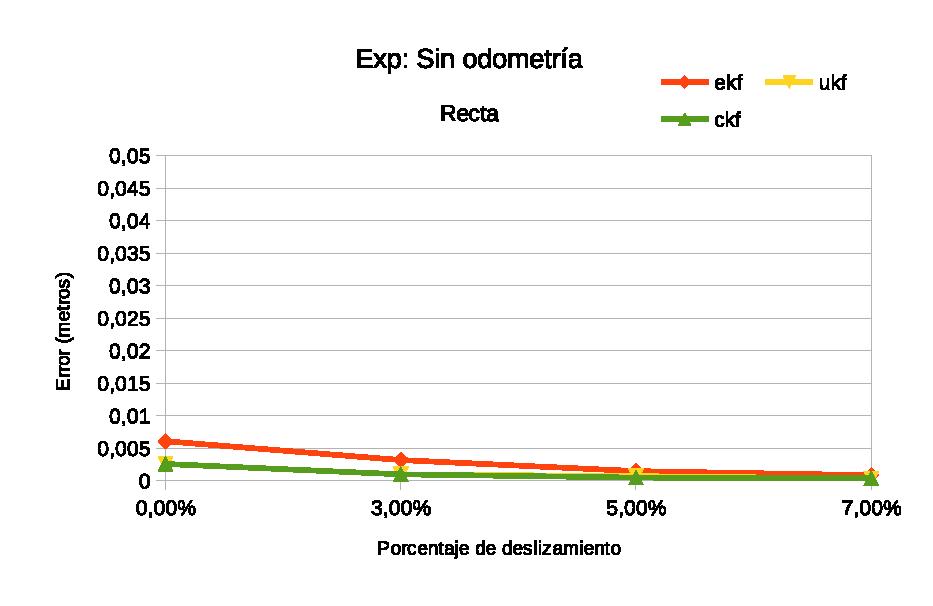
\includegraphics[scale=0.6]{Grafico1_1}
\caption{Experimento recta sin odometría} \label{Grafico1_1}
\end{figure}
\begin{figure}[ht!]
\centering
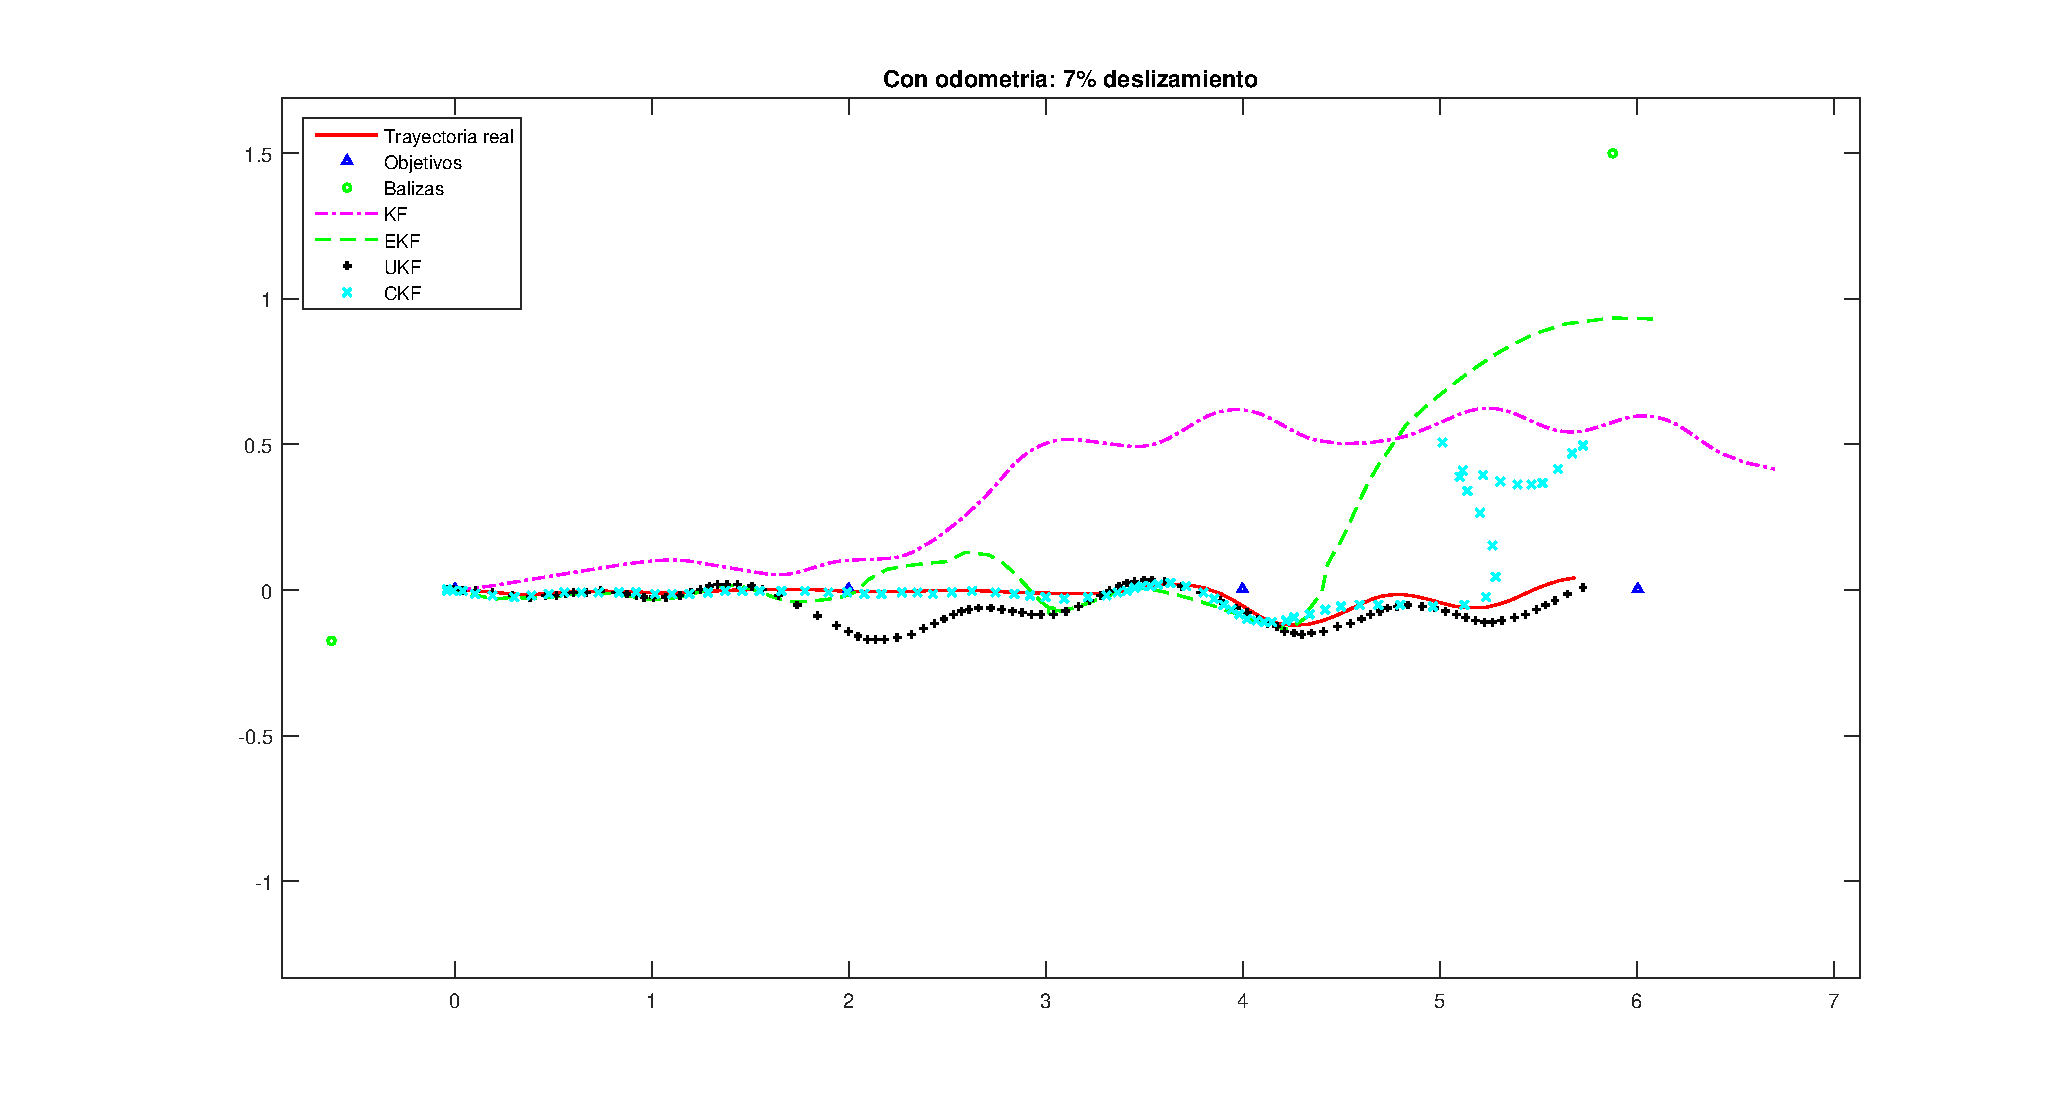
\includegraphics[scale=0.4]{Figura_Recta_Odometria}
\caption{Trayectoria recta con odometría} \label{Figura1}
\end{figure}

\begin{figure}[ht!]
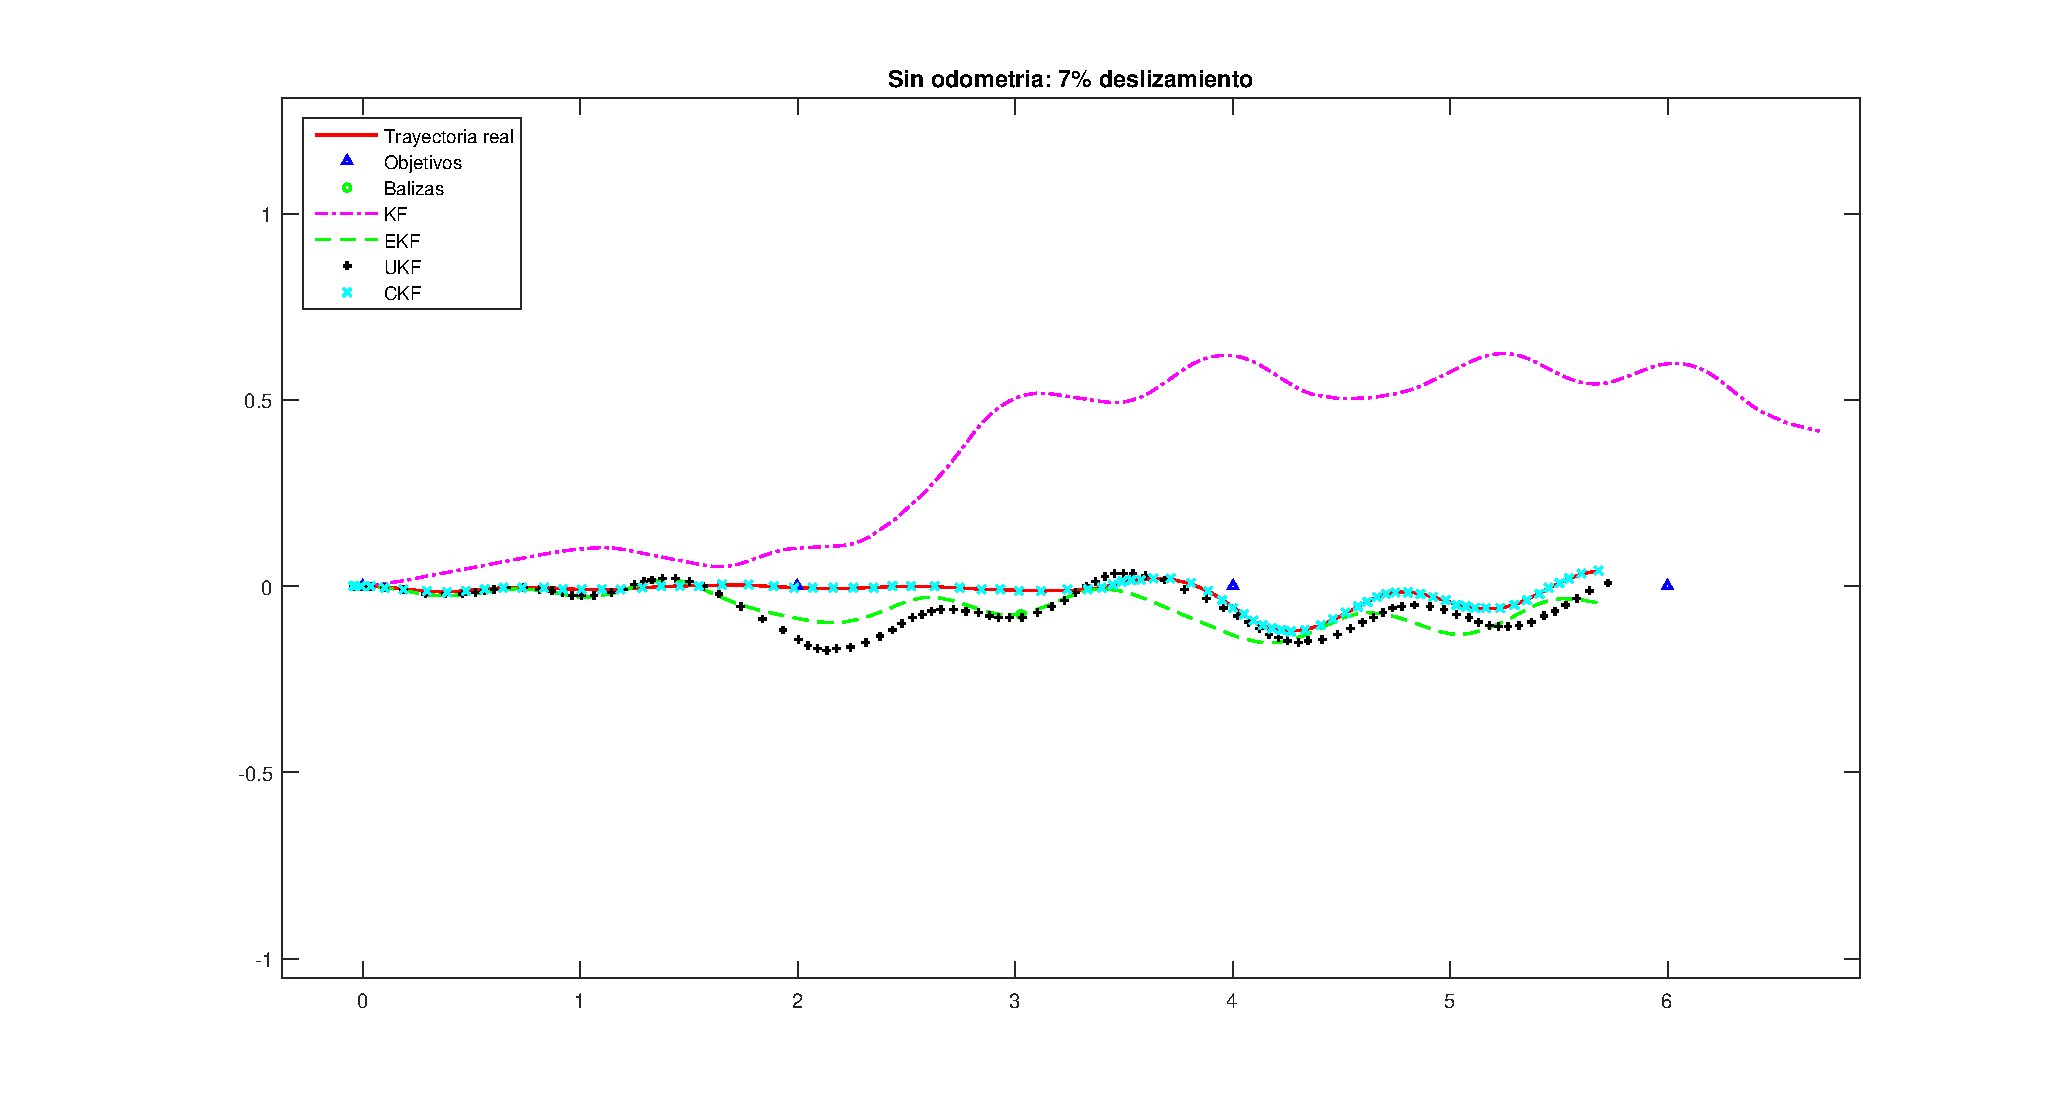
\includegraphics[scale=0.4]{Figura_Recta_SinOdometria}
\caption{Trayectoria recta sin odometría} \label{Figura1_1}
\end{figure}

En las figuras \ref{Grafico1}, \ref{Figura1}, \ref{Grafico1_1} y \ref{Figura1_1}, podemos ver los resultados obtenidos para las dos tandas de experimentos, es decir, con y sin odometría.
Vemos que en ambos casos el \ac{UKF} es el que presenta el menor error, seguido del \ac{CKF} y posteriormente por el \ac{EKF}.
Con respecto al filtro clásico de Kalman vemos que su estimación no es del todo correcta, aunque el error para el 7\% de deslizamiento es de 0.93 metros, y si pensamos que solamente hemos tenido en cuenta la odometría para la estimación este valor no es tan malo.
Otra observación interesante entre las figuras \ref{Grafico1} y \ref{Grafico1_1} es que cuando no implementamos la odometría la estimación es mejor.
Esto es debido a que los deslizamientos hacen que la odometría no sea una información válida y por lo tanto en ese caso sería mejor no implementarla como demuestra la figura \ref{Grafico1_1} donde el máximo error obtenido es de 0.006 metros, lo que significa que hemos tenido una estimación casi perfecta.
% * <amorellg@ull.edu.es> 2016-06-06T19:55:49.119Z:
%
% > Esto es debido a que los deslizamientos hacen que la odometría no sea una información válida y por lo tanto en ese caso sería mejor no implementarla como demuestra la figura \ref{Grafico1_1} donde el máximo error obtenido es de 0.006 metros, lo que significa que hemos tenido una estimación casi perfecta.
%
% Agrupa mejor las gráficas y figuras por su naturaleza, para que sea más fácil comparar el error con y sin odometría y la gráfica de la trayectoria con y sin odometría
%
% ^ <alu0100765755@ull.edu.es> 2016-06-07T09:29:54.802Z:
%
% Hecho !!
%
% ^ <alu0100765755@ull.edu.es> 2016-06-07T09:29:56.442Z.
Es muy importante tener en cuenta que las trayectorias reales mostradas en las figuras \ref{Figura1} y \ref{Figura1_1} no son las trayectorias que han seguido todos los filtros ya que al trabajar con deslizamientos para cada filtro la trayectoria se ha podido ver afectada de distinta manera (por ejemplo si el robot ha deslizado en otra dirección), por esta razón hemos realizado baterías de experimentos y luego hemos obtenido la media del error, con lo cual la trayectoria mostrada es meramente orientativa para saber la forma de la ruta tomada por nuestro robot y no como referencia comparativa.
% * <amorellg@ull.edu.es> 2016-06-06T19:57:13.535Z:
%
% >  figuras \ref{Figura1} y
%
% en la figura 2.8 del error sin odometría, la escala del error es demasiado pequeña y parece que haya más diferencia, cuando estamos hablando del 3er decimal, en la frontera del error numérico del motor de física...  Mira a ver cómo queda poniéndolo 
%
% ^ <alu0100765755@ull.edu.es> 2016-06-07T09:35:01.212Z:
%
% Cambiamos el tamaño de los ejes y listo !
%
% ^ <alu0100765755@ull.edu.es> 2016-06-07T09:43:10.111Z.
\subsection{Resultados para la trayectoria cuadrada}
Para las trayectorias cuadradas la configuración ha sido la misma que para las rectas, los resultados se muestran en las figuras \ref{Grafico2}, \ref{Figura2}, \ref{Grafico2_2} y \ref{Figura2_2}.
\begin{figure}[ht!]
\centering
\includegraphics[scale=0.6]{Grafico2}
\caption{Experimento cuadrado con odometría} \label{Grafico2}
\end{figure}
\begin{figure}[ht!]
\centering
\includegraphics[scale=0.6]{Grafico2_2}
\caption{Experimento cuadrado sin odometría} \label{Grafico2_2}
\end{figure}
\begin{figure}[ht!]
\centering
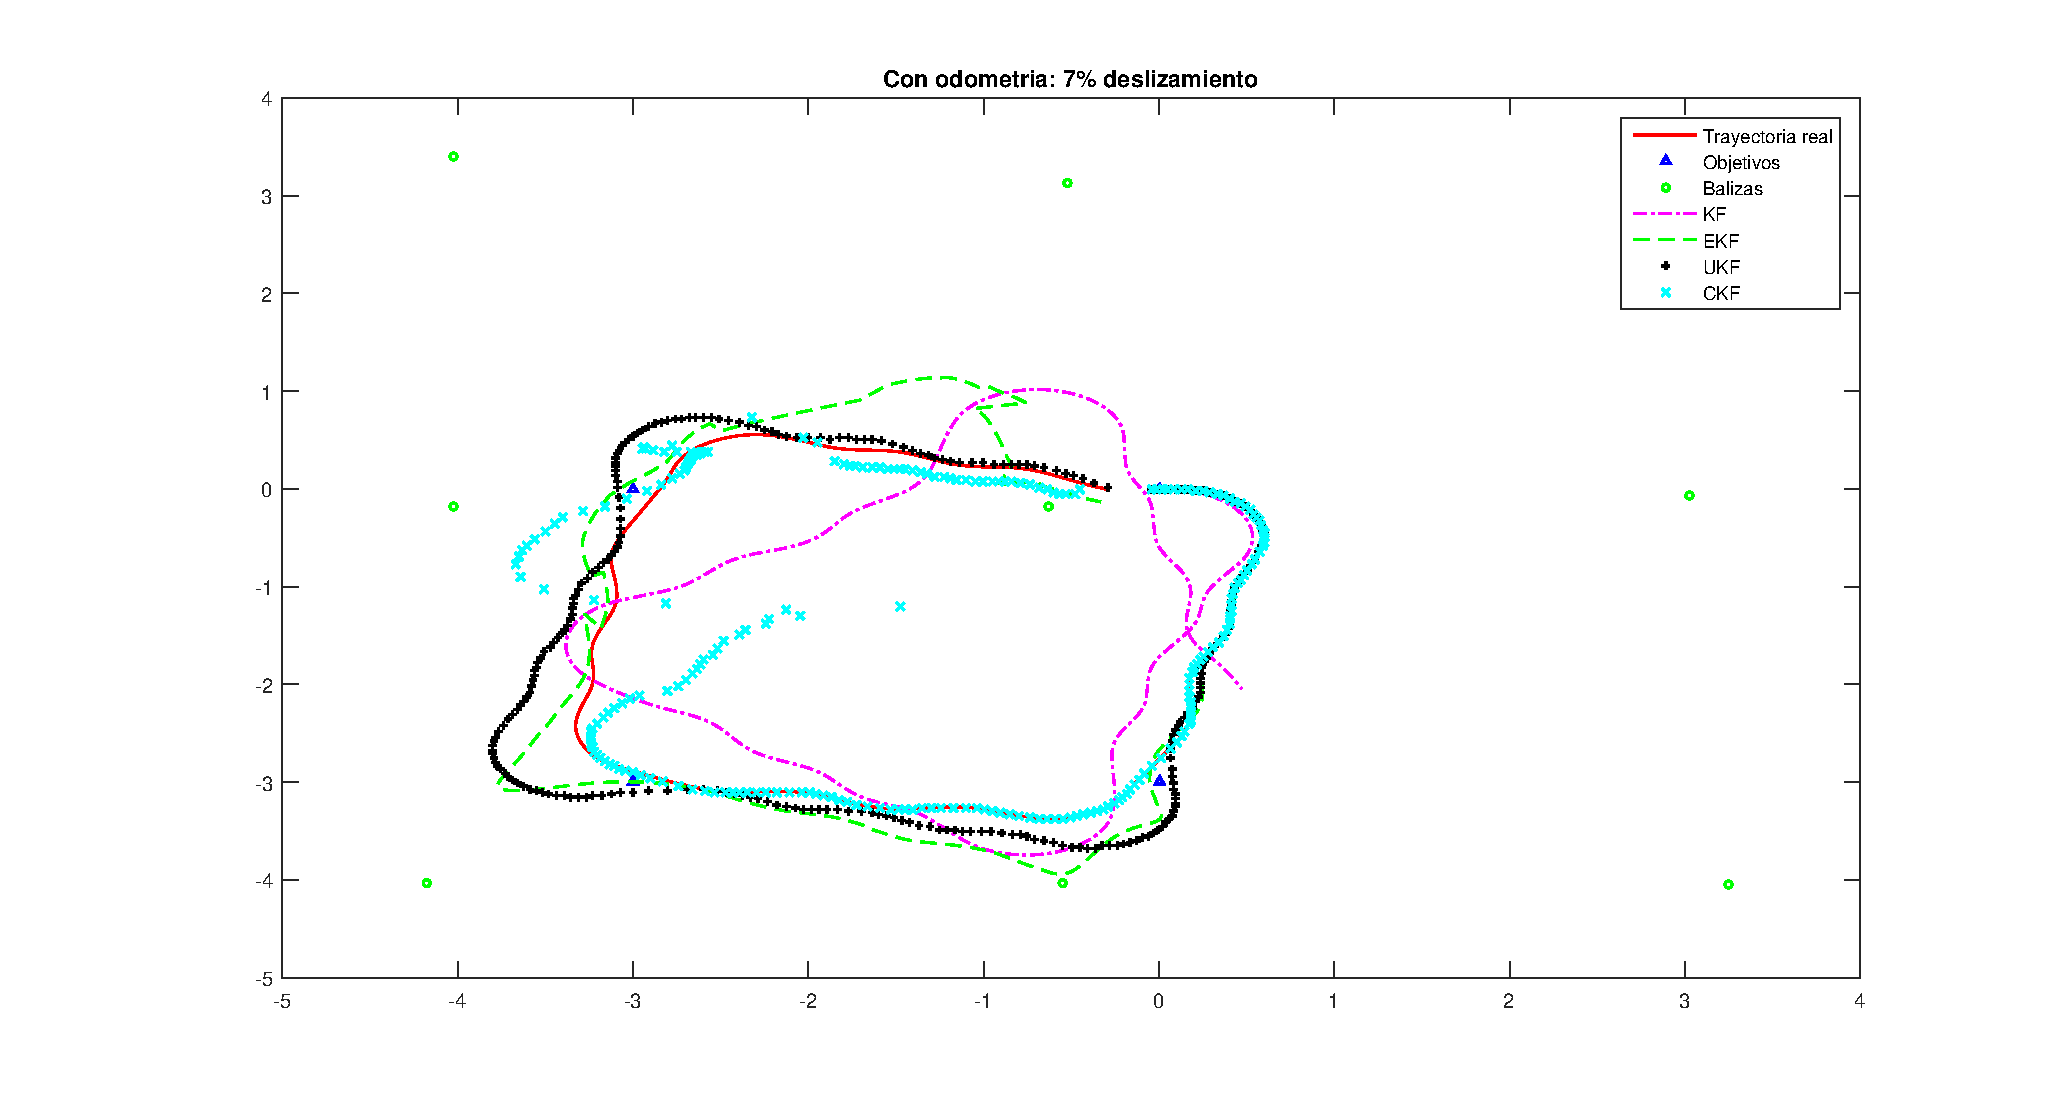
\includegraphics[scale=0.4]{Figura_Cuadrado_Odometria}
\caption{Trayectoria cuadrada con odometría} \label{Figura2}
\end{figure}
\begin{figure}[ht!]
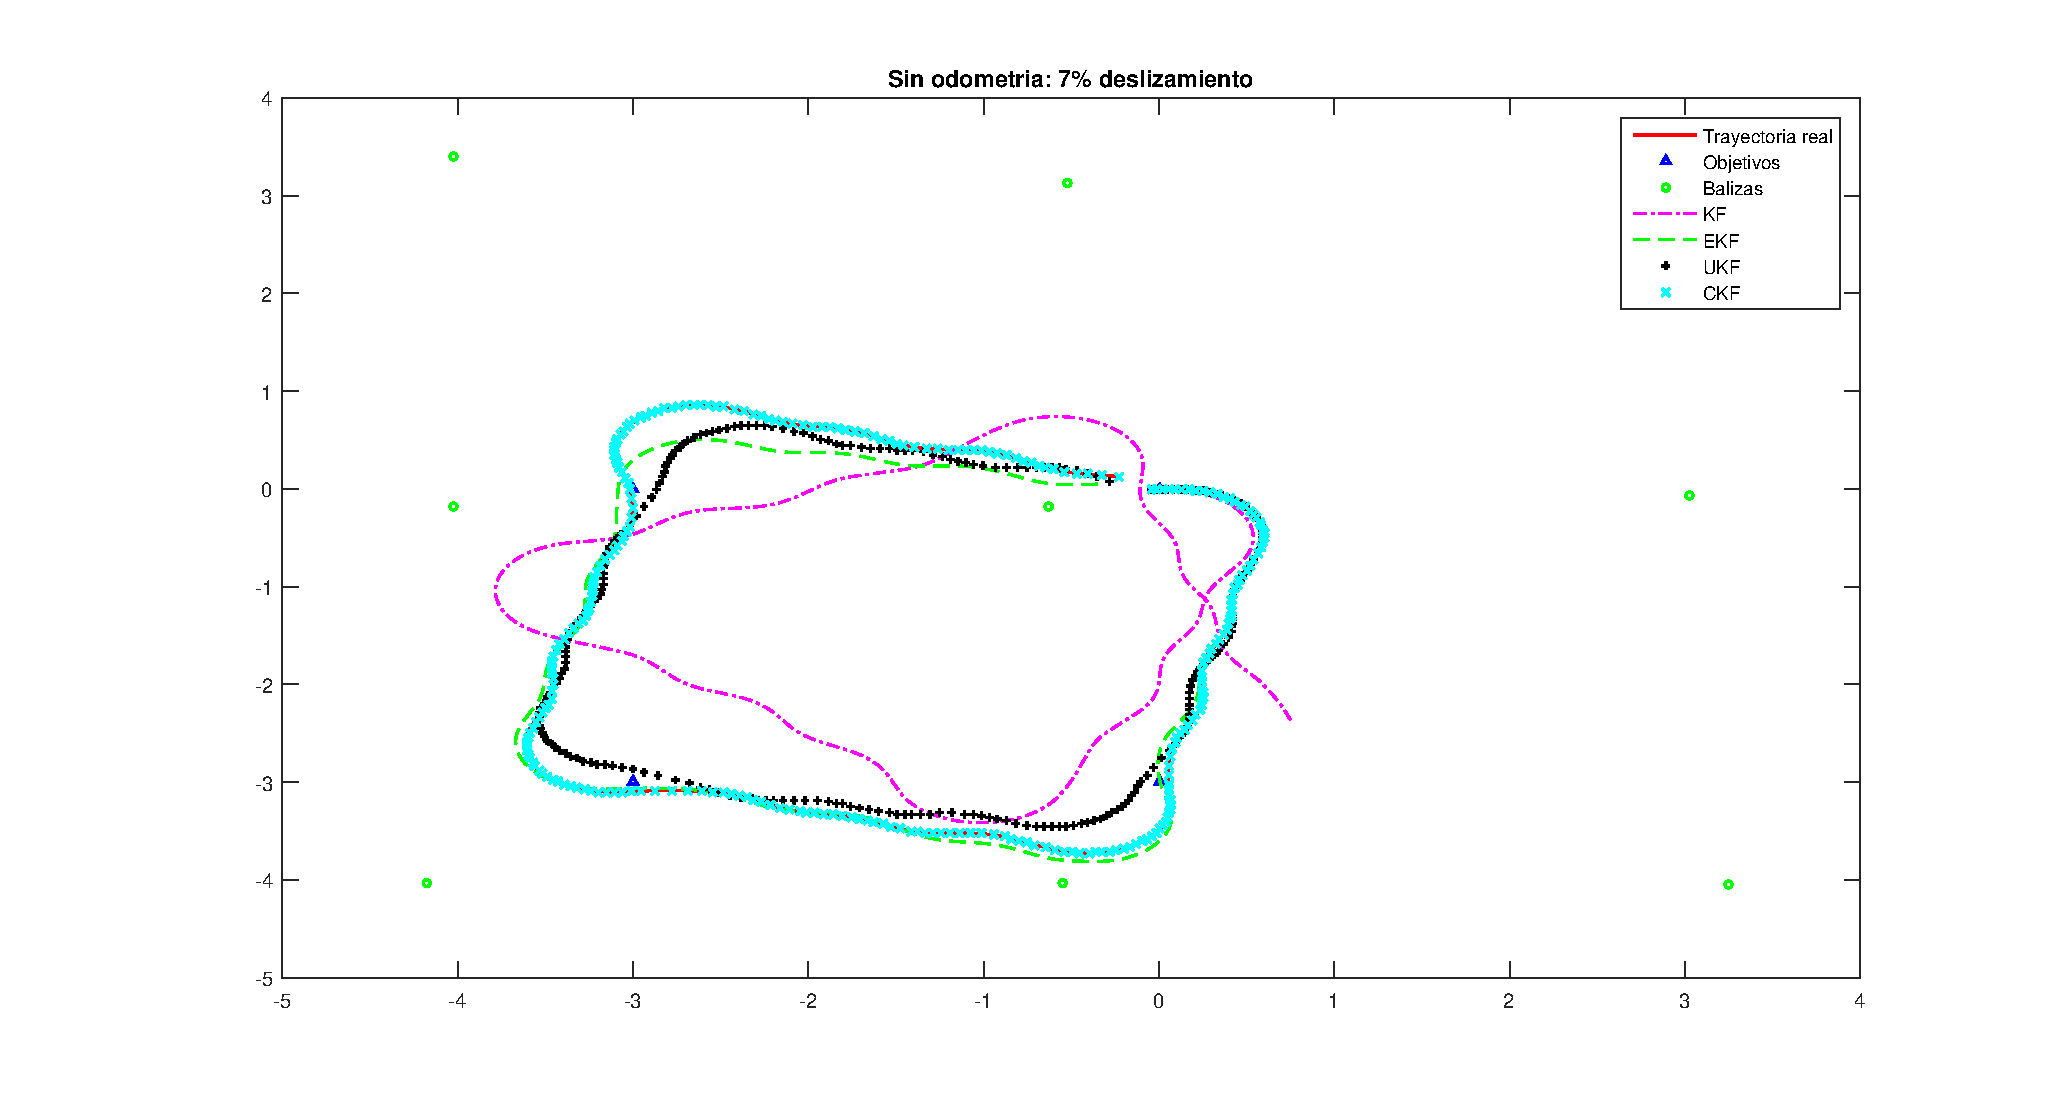
\includegraphics[scale=0.4]{Figura_Cuadrado_SinOdometria}
\caption{Trayectoria cuadrada sin odometría} \label{Figura2_2}
\end{figure}
En este experimento llegamos a unas conclusiones muy parecidas a las del experimento de las rectas.
Vemos que los resultados en la implementación de la odometría \ref{Grafico2} resulta más errónea a medida que el deslizamiento aumenta.
En cambio cuando no implementamos la odometría los errores obtenidos son muy ínfimos como vemos en la figura \ref{Grafico2_2}.
En este experimento el filtro que ha presentado el error más bajo ha sido el \ac{EKF} en el experimento sin la implementación de la odometría como vemos en la figura \ref{Grafico2_2}.
\subsection{Resultados para la trayectoria senoidal}
Los resultados de este experimento son mostrados en las figuras \ref{Grafico3}, \ref{Figura3}, \ref{Grafico3_3} y \ref{Figura3_3}.
\begin{figure}[ht!]
\centering
\includegraphics[scale=0.6]{Grafico3}
\caption{Experimento seno con odometría} \label{Grafico3}
\end{figure}
\begin{figure}[ht!]
\centering
\includegraphics[scale=0.6]{Grafico3_3}
\caption{Experimento seno sin odometría} \label{Grafico3_3}
\end{figure}
\begin{figure}[ht!]
\centering
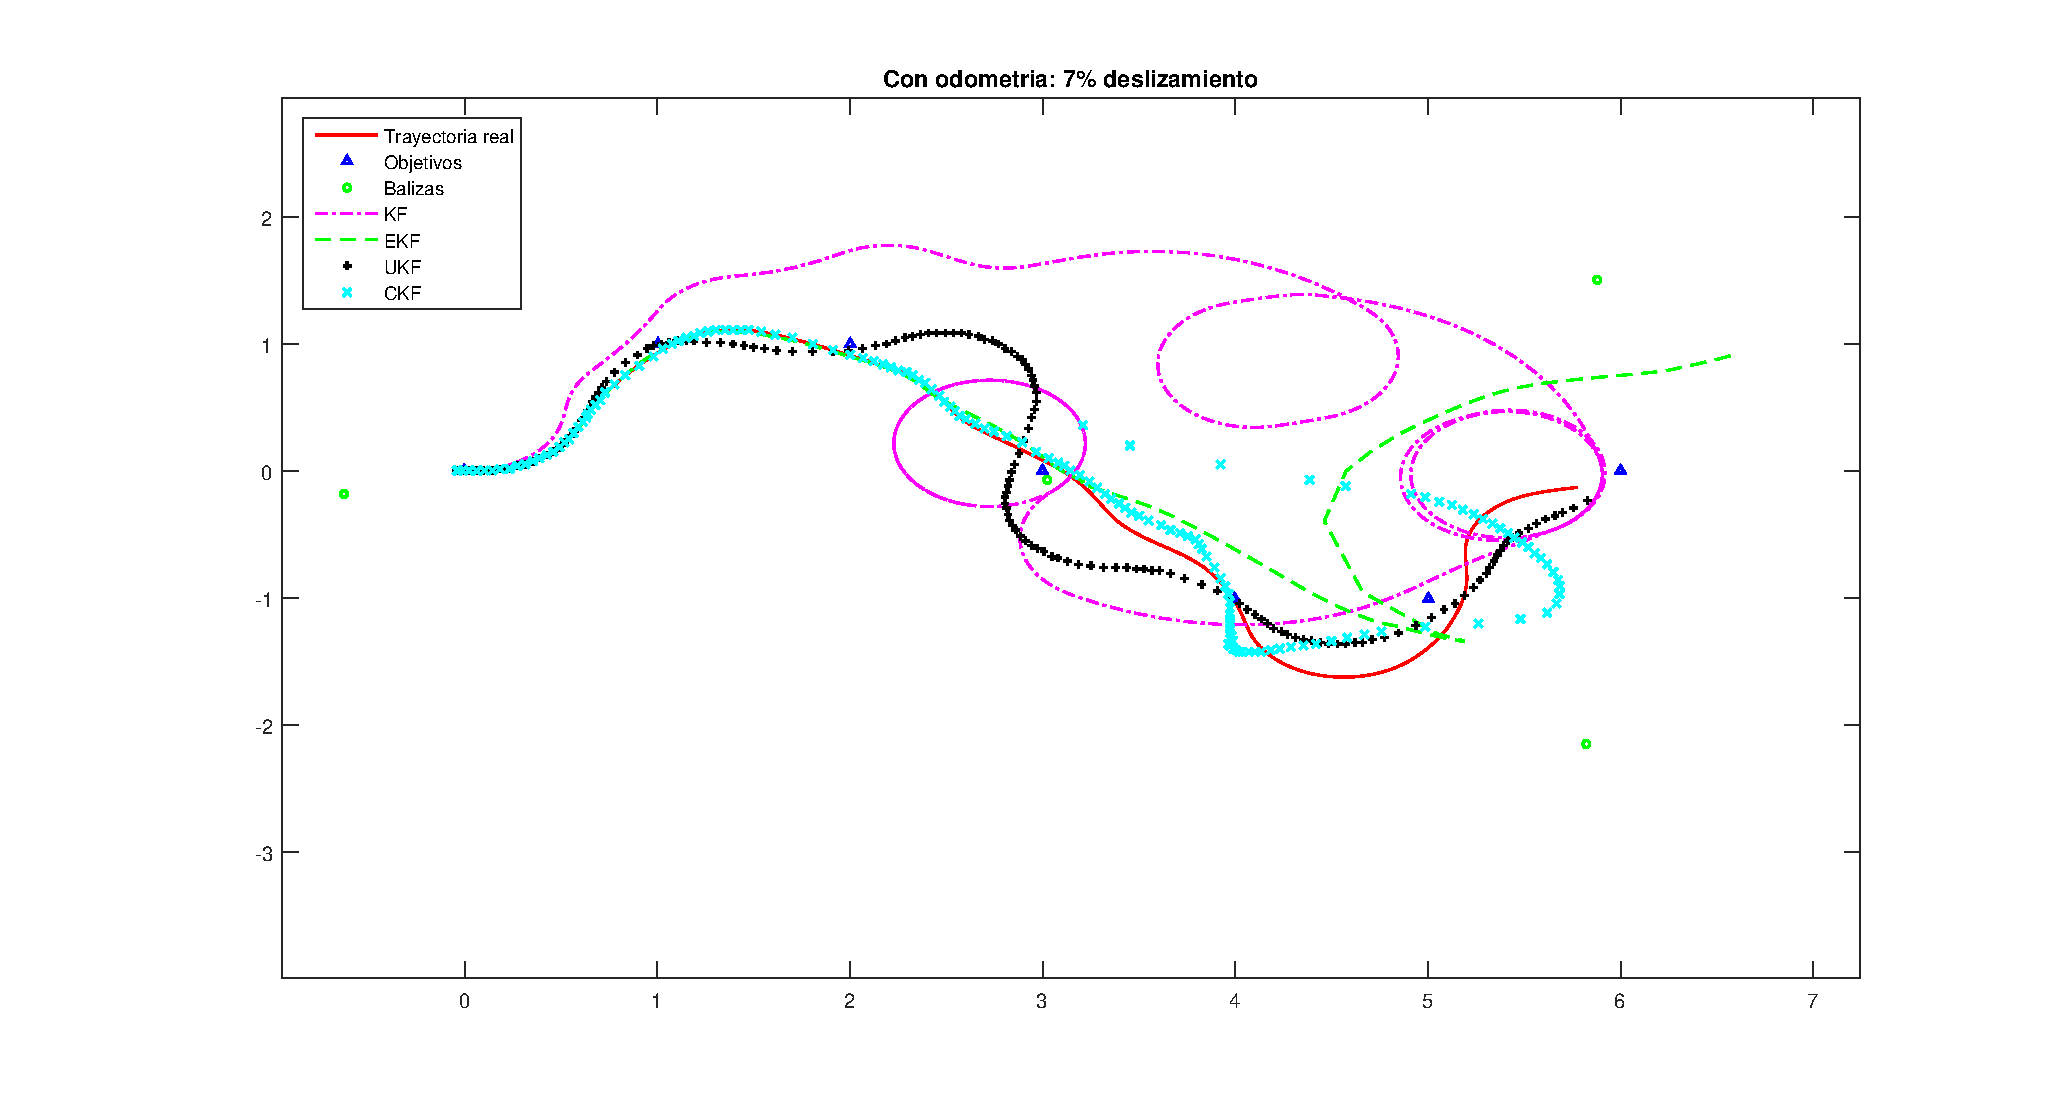
\includegraphics[scale=0.4]{Figura_Seno_Odometria}
\caption{Trayectoria senoidal con odometría} \label{Figura3}
\end{figure}

\begin{figure}[ht!]
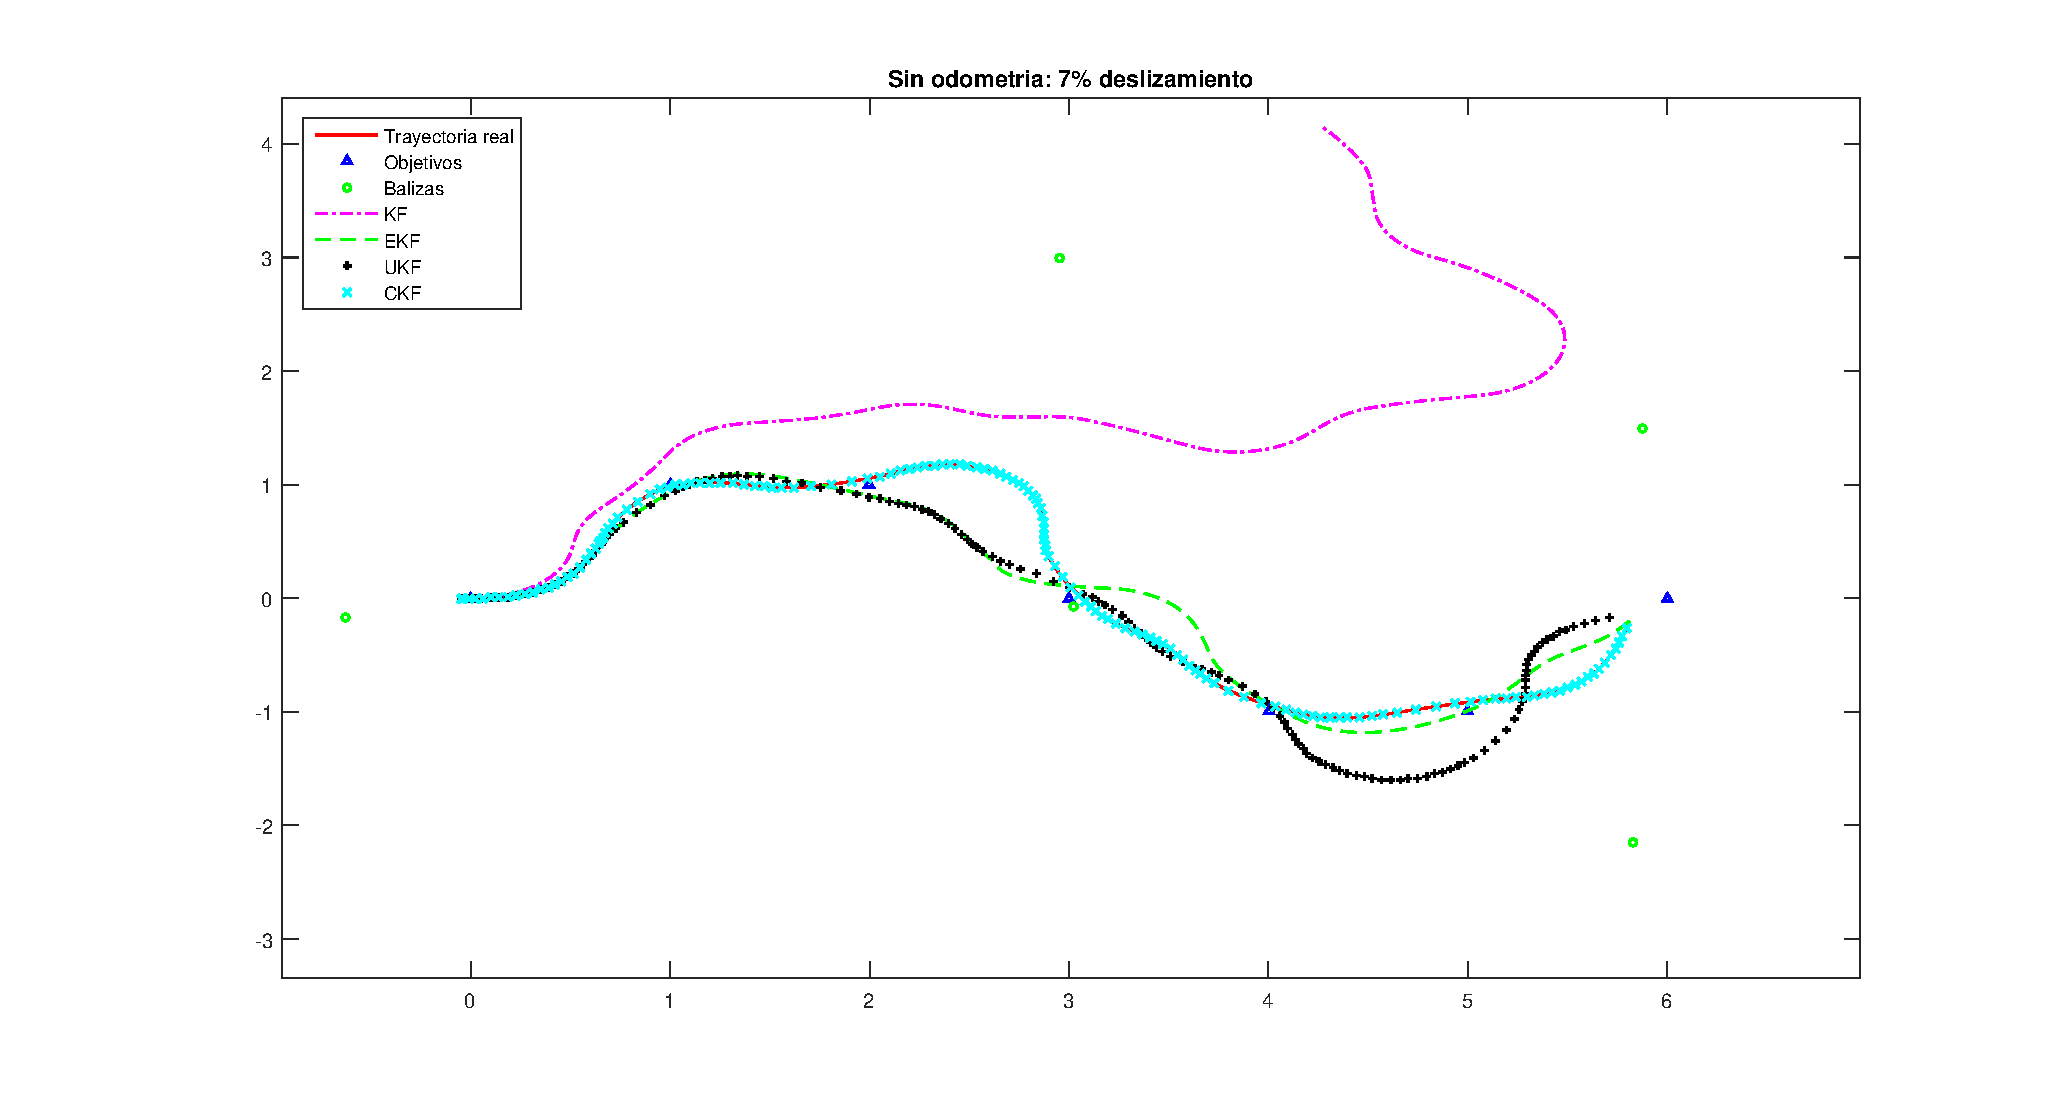
\includegraphics[scale=0.4]{Figura_Seno_SinOdometria}
\caption{Trayectoria senoidal sin odometría} \label{Figura3_3}
\end{figure}
Para esta serie de pruebas llegamos a las mismas conclusiones que para todas las anteriores, por lo que podemos concluir que la odometría puede ser una información peligrosa si trabajamos con deslizamientos muy grandes.
Por otra parte hay que notar que en las figuras \ref{Figura3} y \ref{Figura3_3} el filtro claśico de Kalman tiene un comportamiento muy diferente e igualmente erróneo, esto es debido a que en cada simulación el motor de físicas del simulador hace que el robot pueda deslizar más o menos en distintas zonas además de que nuestro planificador de rutas puede llegar a tomar diferentes decisiones en función de los deslizamientos, por esta razón el aspecto de la simulación es diferente y no debemos tomar las trayectorias mostradas en las figuras \ref{Figura3} y \ref{Figura3_3} como representación de la serie de experimentos, estas figuras son meramente orientativas y escogidas al azar dentro de la serie de pruebas realizadas.

La conclusión para esta serie de experimentos es la siguiente: \textbf{La odometría es una información que puede ayudar a localizarnos con éxito, pero con la existencia de deslizamientos puede ocurrir que esta información contribuya a la deslocalización.}

\section{Experimento 2: Ruido en las medidas}
En esta sección de experimentos veremos como afecta el ruido en los sensores a la estimación que realizan los filtros.
Representaremos los resultados por medio de gráficos para una mejor comprensión y análisis de estos.
Además representaremos las trayectorias seguidas por los filtros para el peor caso de estimación y usaremos dos funciones de medida distintas de las que ya hemos hablado: la función de medida de distancia (ecuación \ref{Modelo_distancia}) y la de medida de ángulos (ecuación \ref{Modelo_angulo}).
La sintonización de los filtros y sus parámetros es la misma que para el experimento 1.
Además el deslizamiento se fijará en un $0\%$ para esta serie de pruebas.
% * <amorellg@ull.edu.es> 2016-06-06T20:30:33.632Z:
%
% > .
%
% añade, para recordar: "en estos experimentos fijamos el valor de deslizamiento en XX%"
%
% ^ <alu0100765755@ull.edu.es> 2016-06-07T09:44:54.991Z.
\subsection{Resultados para la trayectoria recta}
En las figuras \ref{Grafico4}, \ref{Figura4}, \ref{Grafico4_4} y \ref{Figura4_4} podemos ver los resultados obtenidos.
\begin{figure}[ht!]
\centering
\includegraphics[scale=0.6]{Grafico4}
\caption{Experimento recta función de medida de distancia} \label{Grafico4}
\end{figure}
\begin{figure}[ht!]
\centering
\includegraphics[scale=0.6]{Grafico4_4}
\caption{Experimento recta función de medida de ángulos} \label{Grafico4_4}
\end{figure}
\begin{figure}[ht!]
\centering
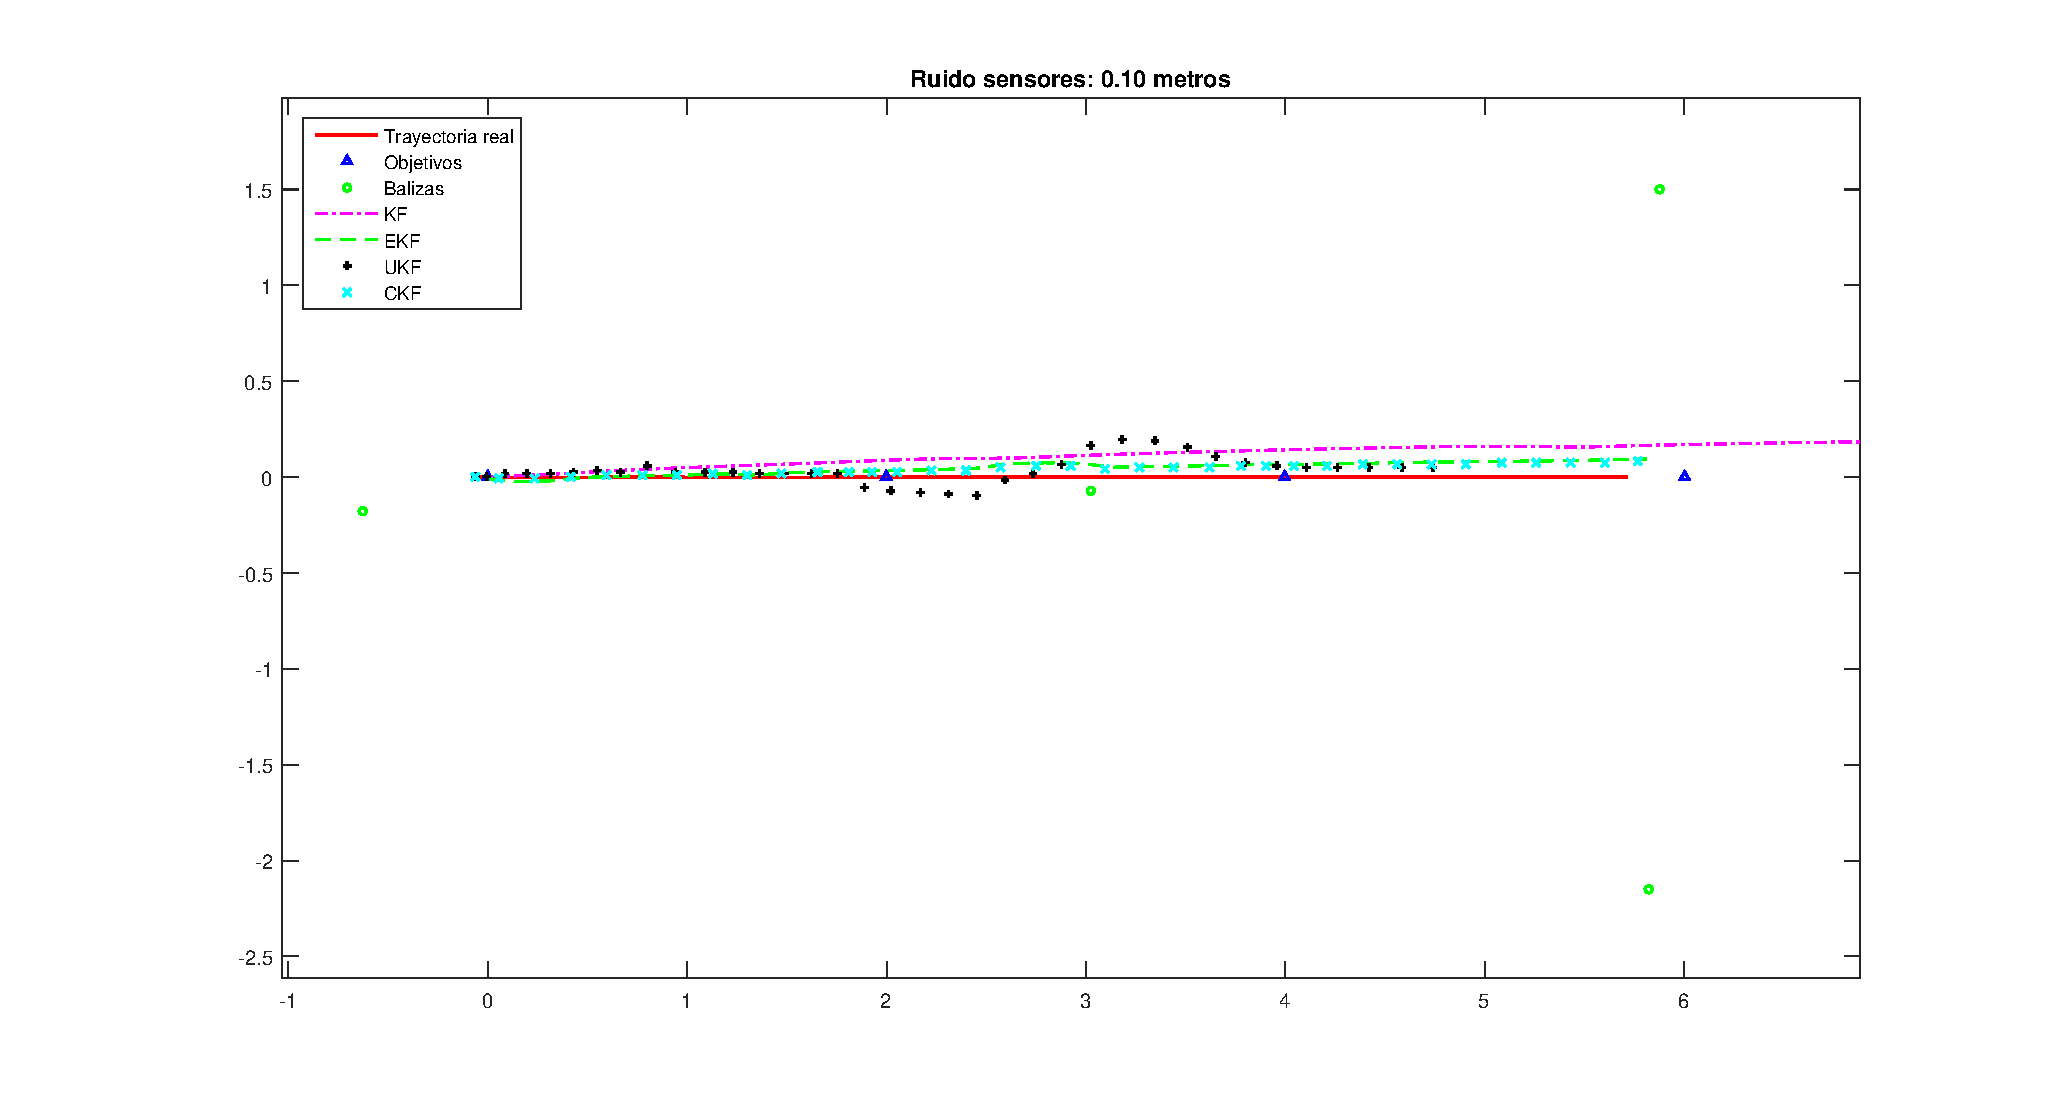
\includegraphics[scale=0.4]{Figura4}
\caption{Trayectoria recta función de medida de distancia} \label{Figura4}
\end{figure}

\begin{figure}[ht!]
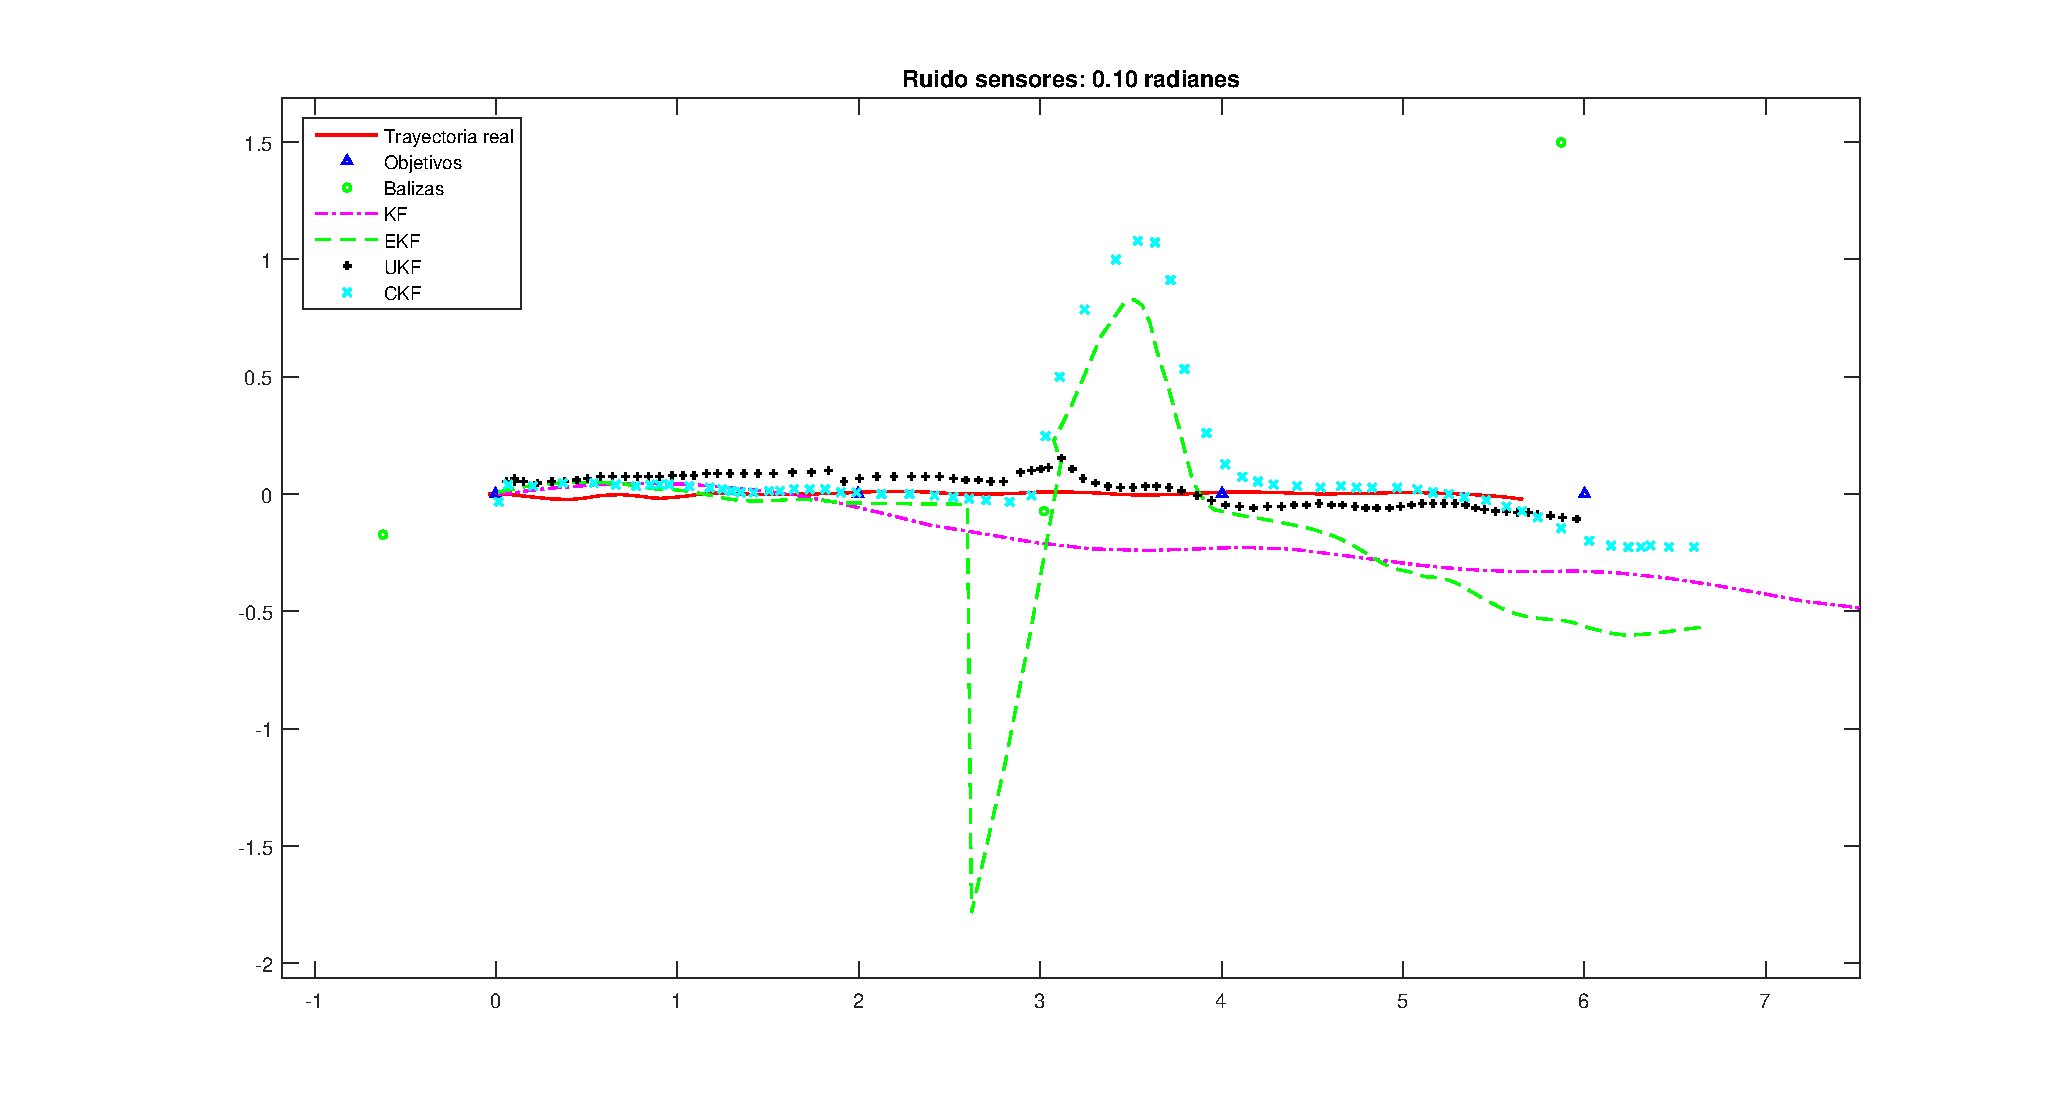
\includegraphics[scale=0.4]{Figura4_4}
\caption{Trayectoria recta función de medida de ángulos} \label{Figura4_4}
\end{figure}
Podemos ver claramente en la figura \ref{Figura4_4} que para el modelo de medida de ángulos existen muchas singularidades que hacen que la estimación sea totalmente errónea, como es el caso del \ac{EKF} o el \ac{UKF} en dicha figura.
Además si comparamos las figuras \ref{Grafico4} y \ref{Grafico4_4} vemos que los errores son más grandes para la función de medida de ángulos que para la función de medida de distancias y algunos casos es debido a las singularidades.
El \ac{CKF} ha sido el filtro que menor error ha tenido en la figura \ref{Grafico4} mientras que para el modelo de medida de ángulos (figura \ref{Grafico4_4}) ha sido el \ac{UKF}.
Por último, como era de esperar el error en la localización tiende a aumentar a medida que aumenta el ruido presente en los sensores, lo cuál es lógico.
También vemos que para el \ac{UKF} es menor el error si la función de medida utilizada es la de ángulos, para el \ac{CKF} y el \ac{EKF} pasa totalmente lo contrario.

\subsection{Resultados para la trayectoria cuadrada}
Las figuras \ref{Grafico5}, \ref{Figura5}, \ref{Grafico5_5} y \ref{Figura5_5} muestran los resultados para esta serie de experimentos.
La configuración utilizada ha sido la misma que para todas las pruebas hasta el momento.
\begin{figure}[ht!]
\centering
\includegraphics[scale=0.6]{Grafico5}
\caption{Experimento cuadrado función de medida de distancia} \label{Grafico5}
\end{figure}
\begin{figure}[ht!]
\centering
\includegraphics[scale=0.6]{Grafico5_5}
\caption{Experimento cuadrado función de medida de ángulos} \label{Grafico5_5}
\end{figure}
\begin{figure}[ht!]
\centering
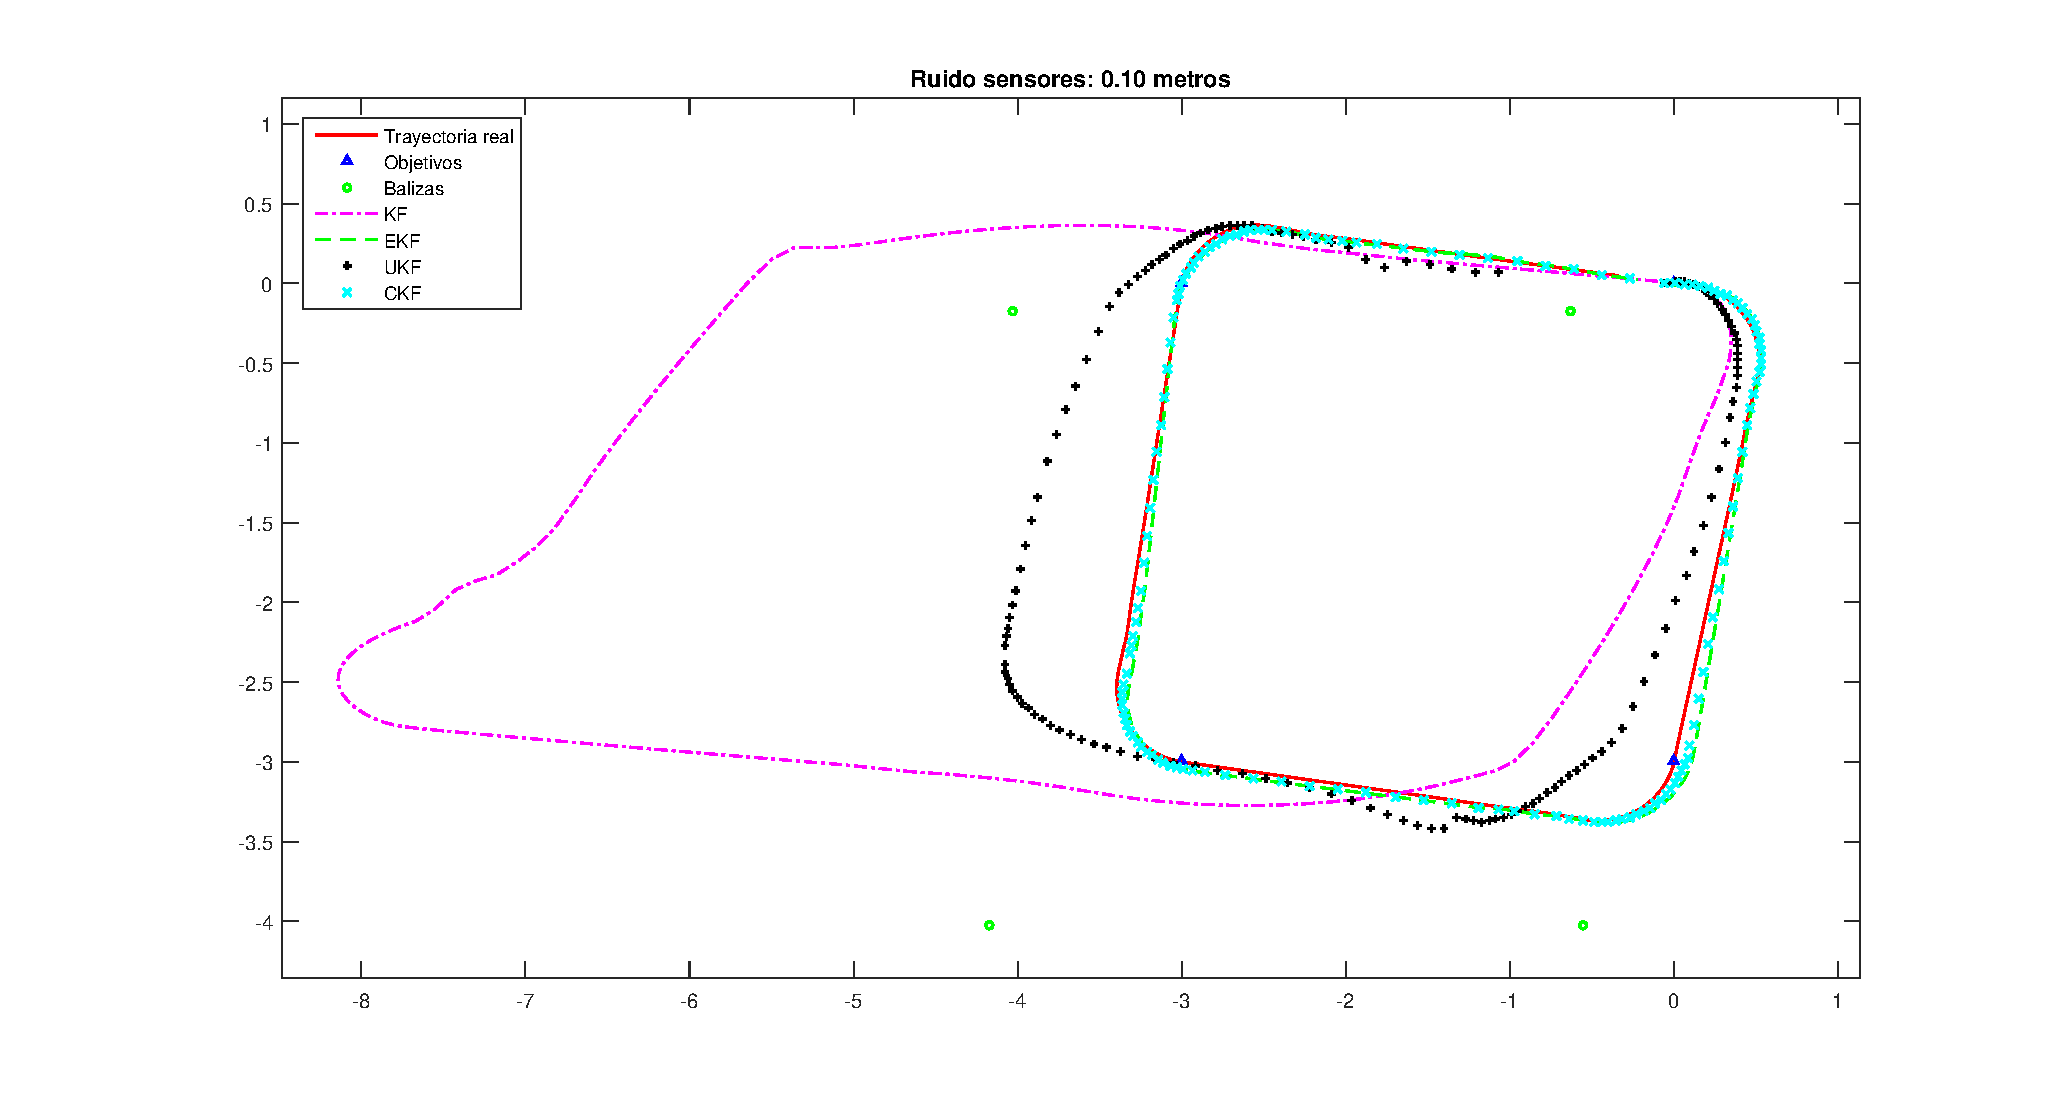
\includegraphics[scale=0.4]{Figura5}
\caption{Trayectoria cuadrada función de medida de distancia} \label{Figura5}
\end{figure}

\begin{figure}[ht!]
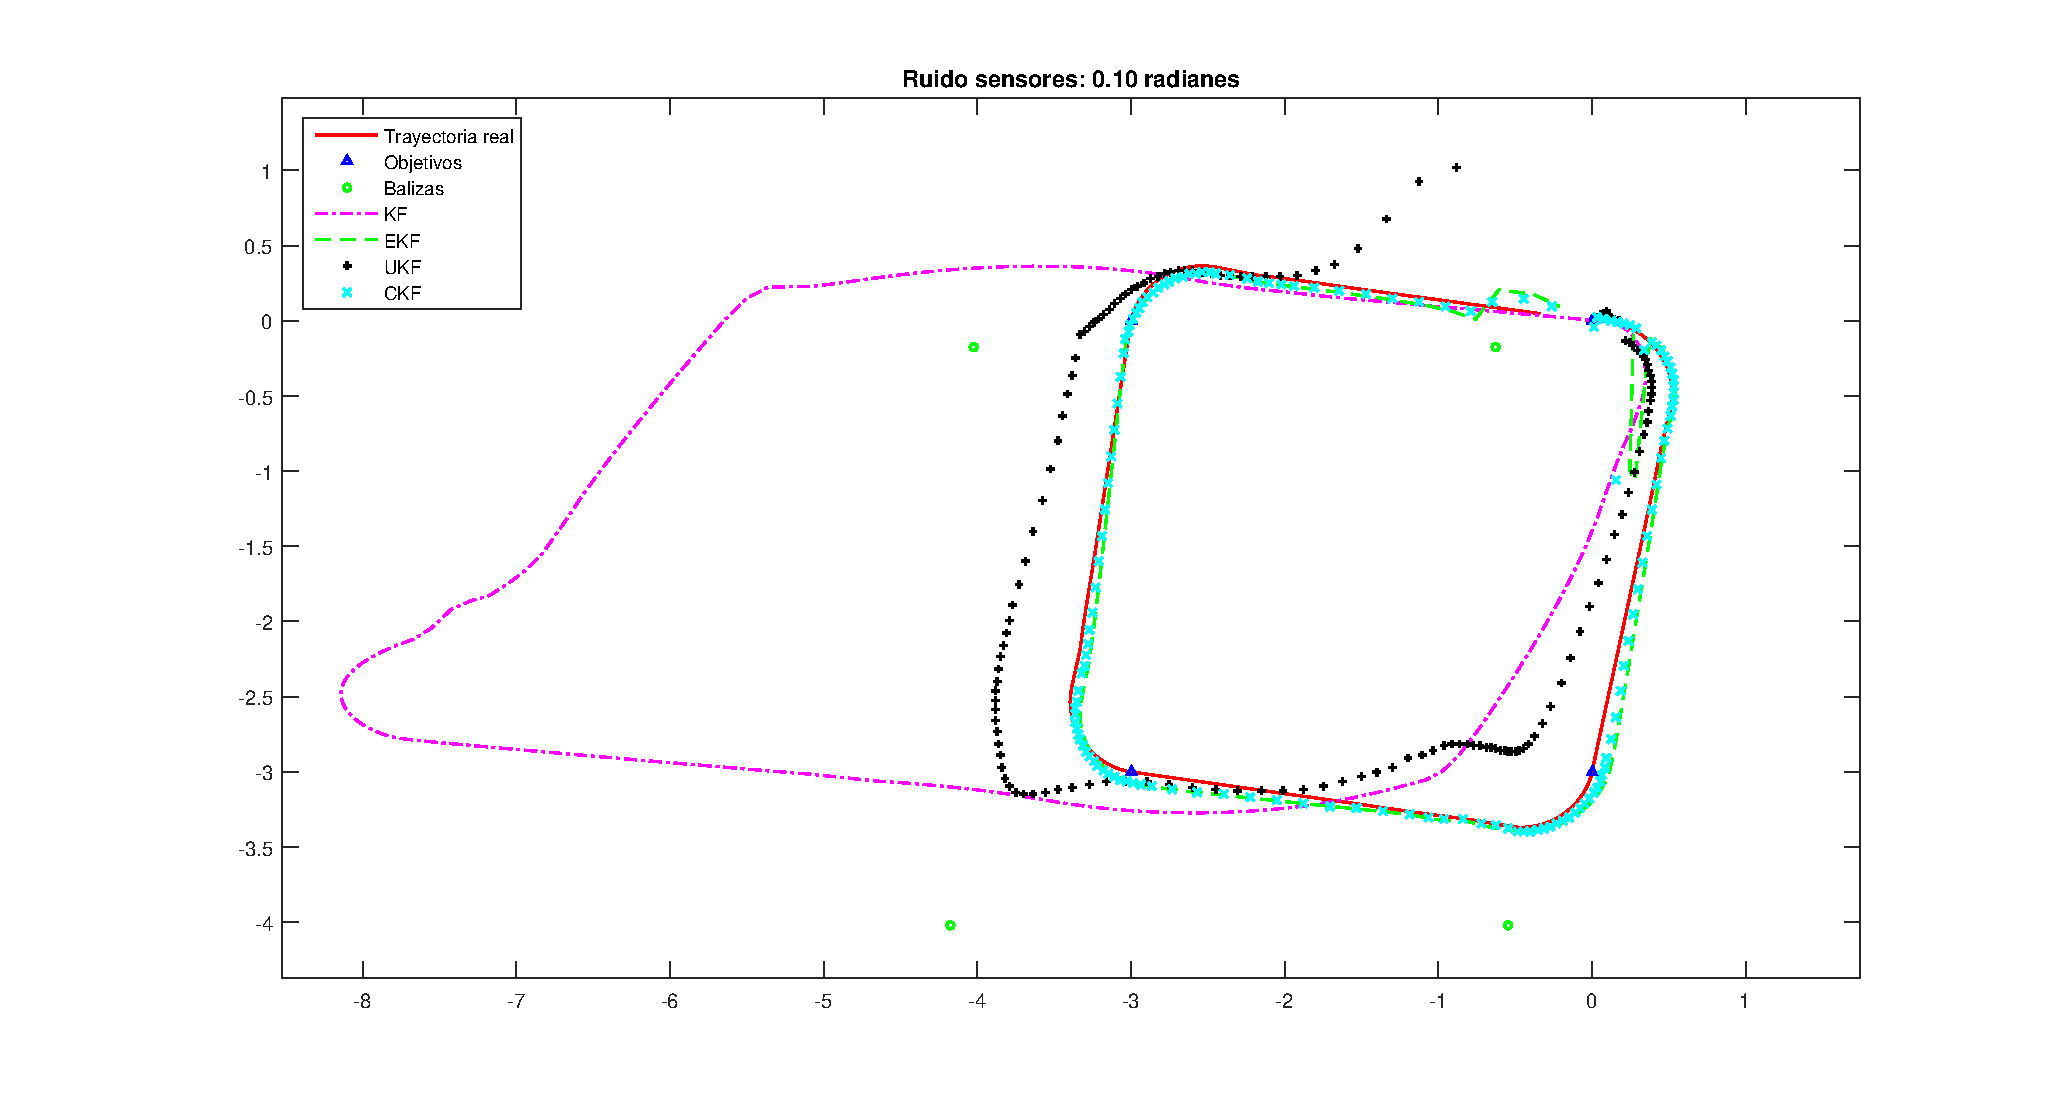
\includegraphics[scale=0.4]{Figura5_5}
\caption{Trayectoria cuadrada función de medida de ángulos} \label{Figura5_5}
\end{figure}
En este caso los resultados se repiten con respecto al primer experimento de esta serie.
Podemos ver que el \ac{UKF} presenta errores mayores cuando usa la función de medida de distancia, además también podemos observar ciertas singularidades en la figura \ref{Figura5_5} provocadas por la función de medida de ángulos.
En \ac{CKF} ha sido el filtro que menor error ha presentado en general.
En la figura \ref{Figura5} vemos como el error aumenta a medida que lo hace el ruido en los sensores, en cambio en la figura \ref{Figura5_5} vemos todo lo contrario y esto es debido a que probablemente para el primer experimento de la serie las singularidades hayan hecho aumentar el error obtenido.
Aun con lo anterior para este caso la función de medida de distancias tiene un mejor comportamiento ya que los errores obtenidos de forma global son menores como vemos en la figura \ref{Grafico5} en comparación con \ref{Grafico5_5}, por lo que se demuestra que la función de medida de distancias es más eficiente que la de medida de ángulos.
\subsection{Resultados para la trayectoria senoidal}
Los resultados de esta serie de experimentos pueden verse en las figuras \ref{Grafico6}, \ref{Figura6}, \ref{Grafico6_6} y \ref{Figura6_6}.
\begin{figure}[ht!]
\centering
\includegraphics[scale=0.6]{Grafico6}
\caption{Experimento seno función de medida de distancia} \label{Grafico6}
\end{figure}
\begin{figure}[ht!]
\centering
\includegraphics[scale=0.6]{Grafico6_6}
\caption{Experimento seno función de medida de ángulos} \label{Grafico6_6}
\end{figure}
\begin{figure}[ht!]
\centering
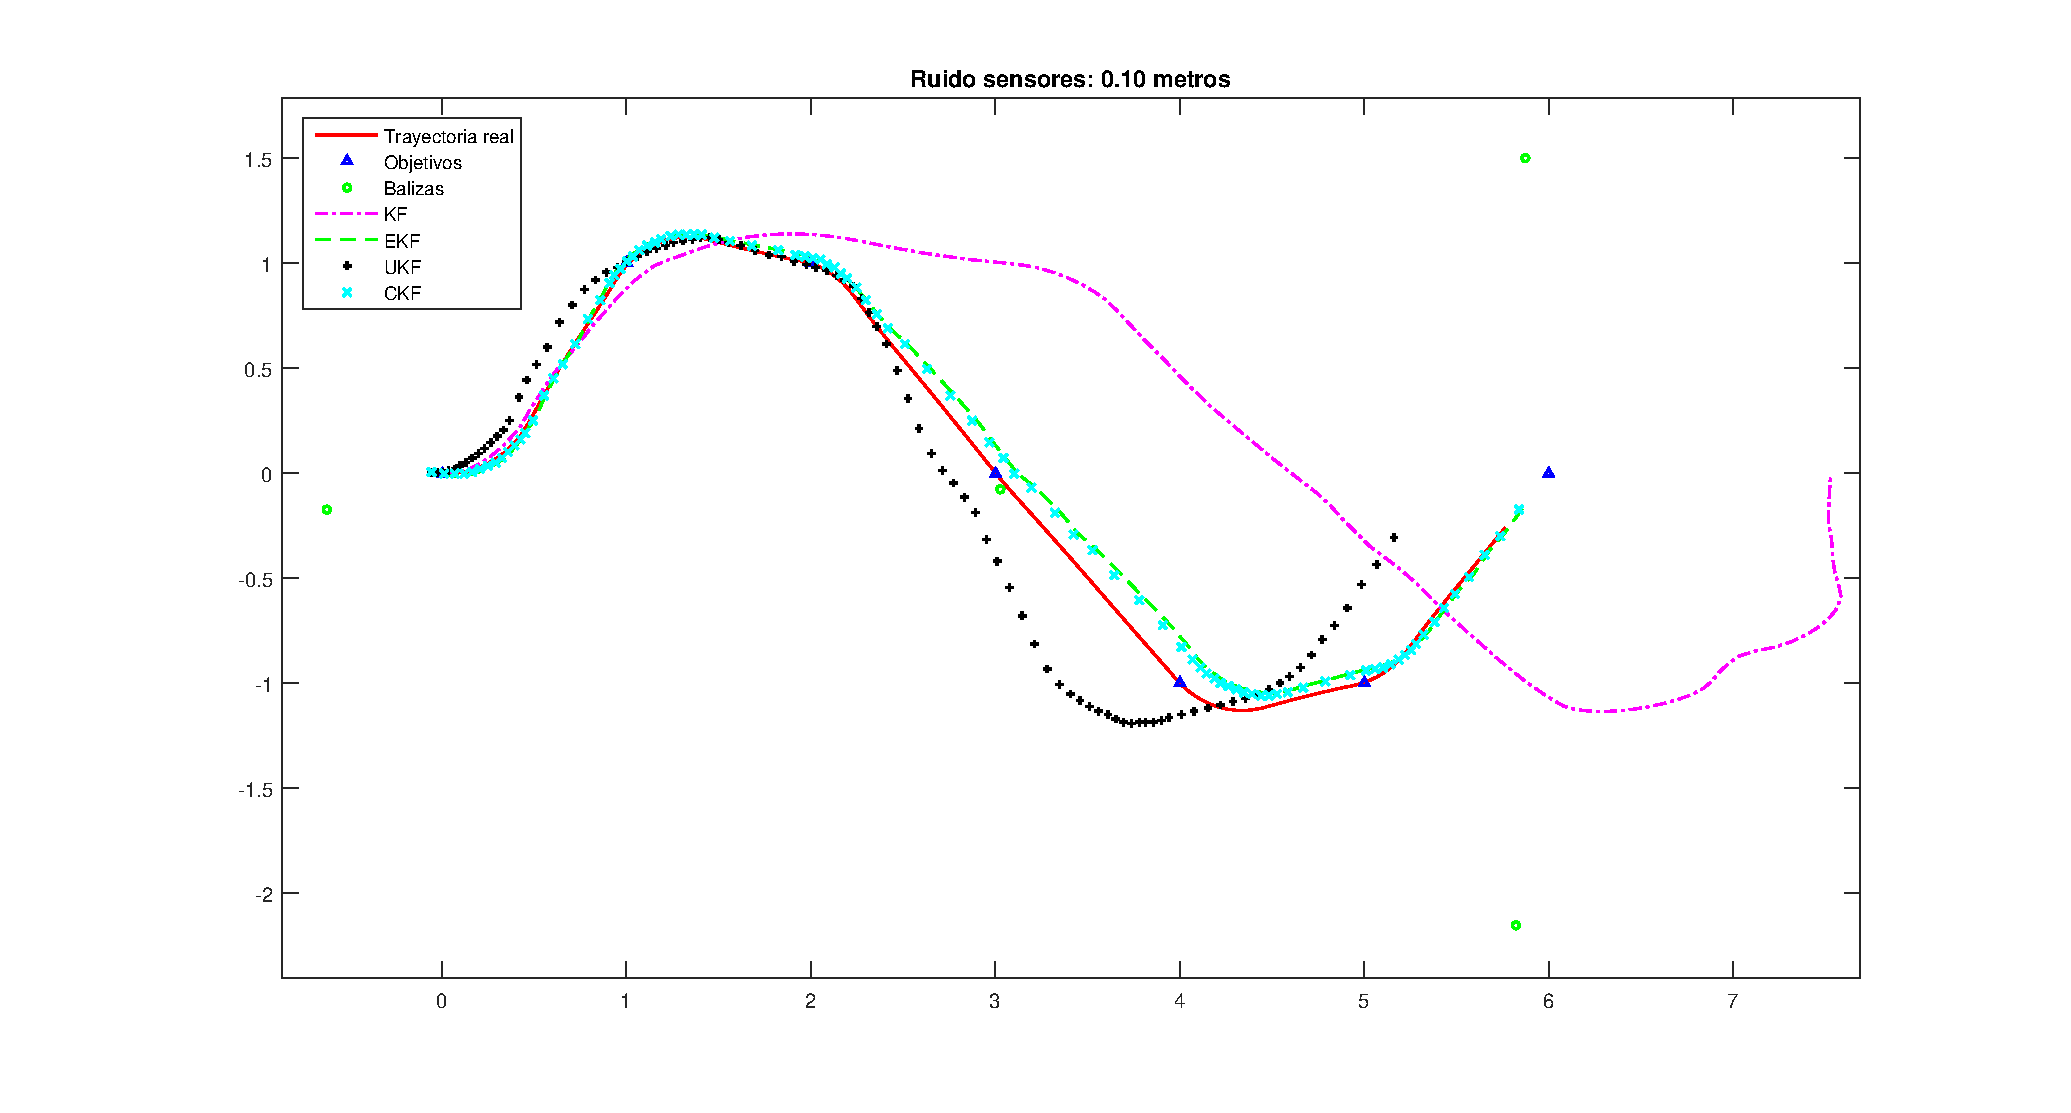
\includegraphics[scale=0.4]{Figura6}
\caption{Trayectoria senoidal función de medida de distancia} \label{Figura6}
\end{figure}

\begin{figure}[ht!]
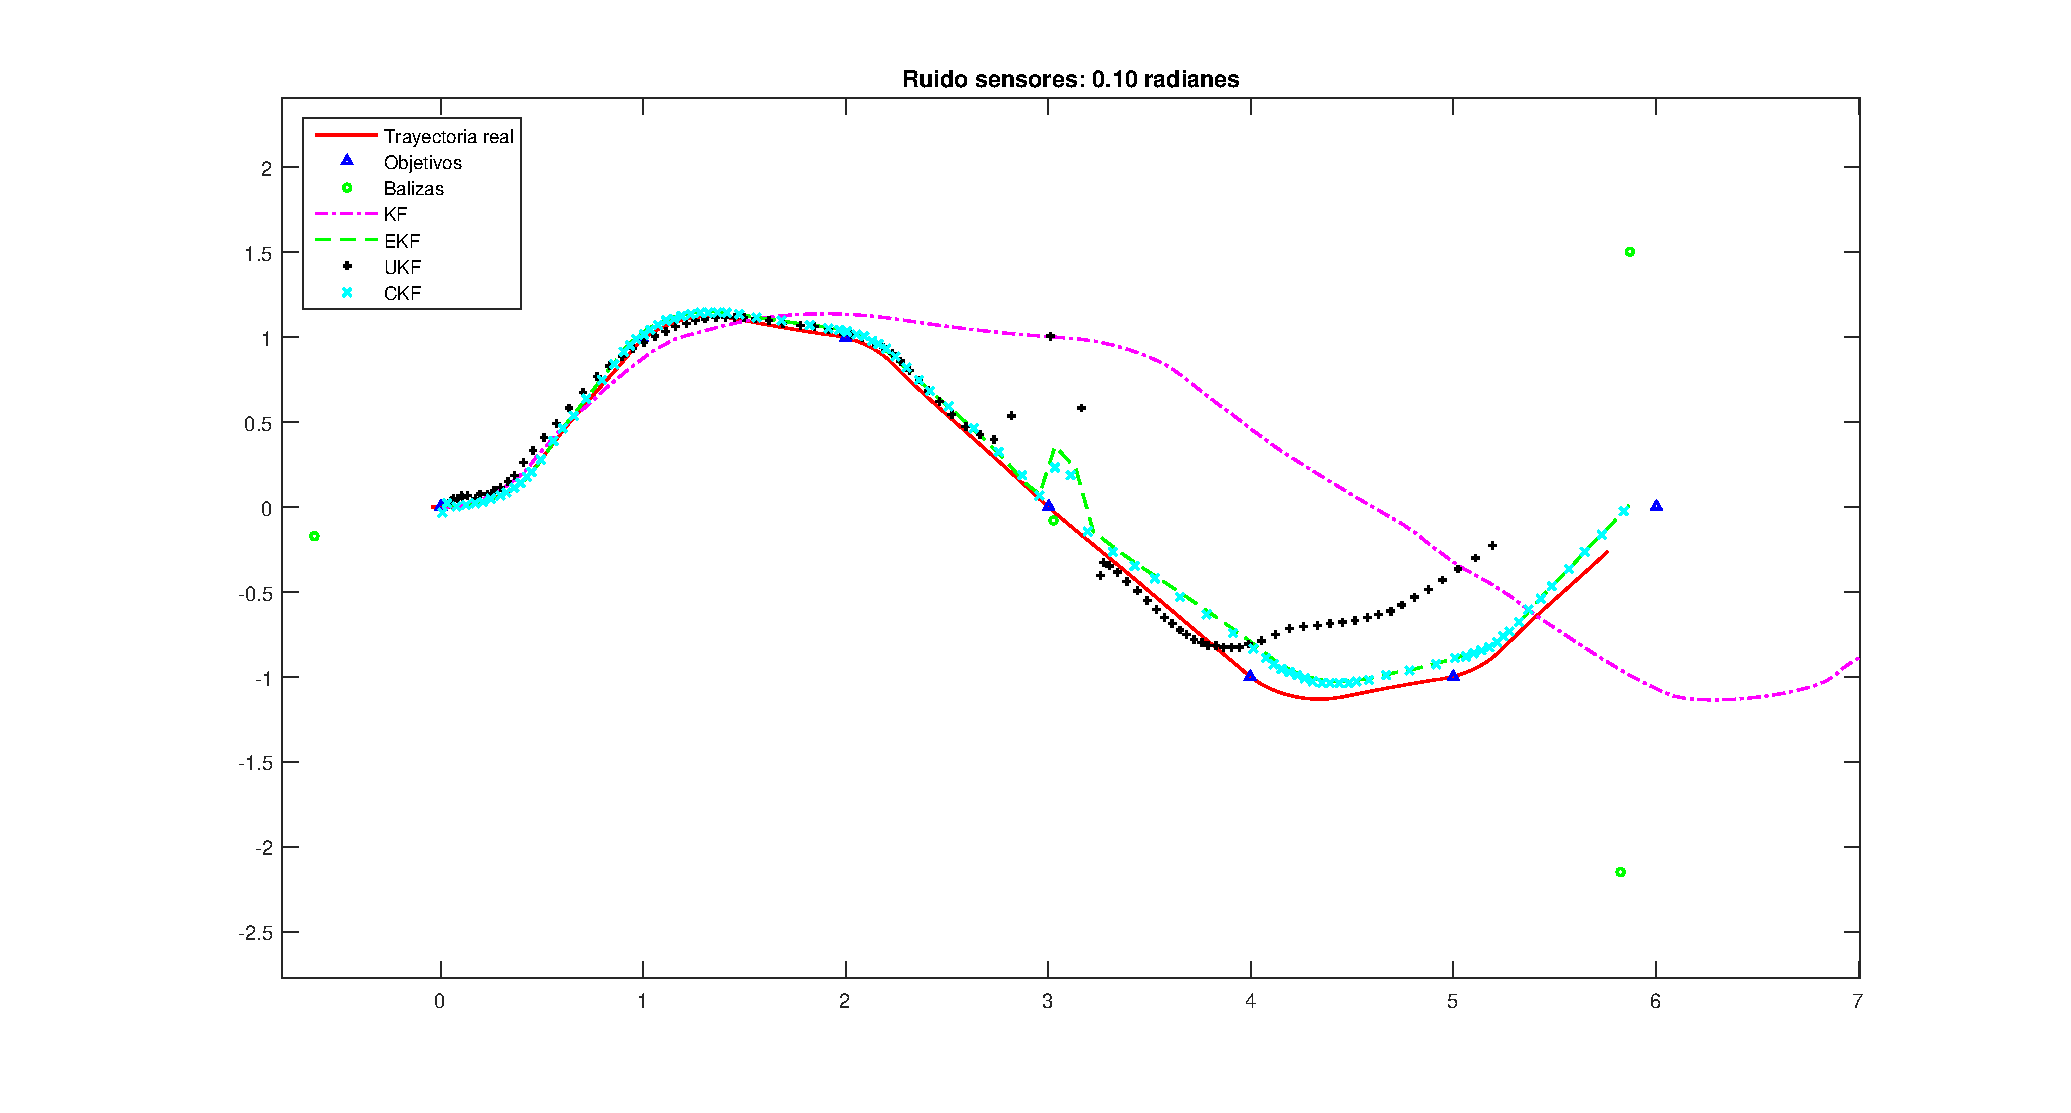
\includegraphics[scale=0.4]{Figura6_6}
\caption{Trayectoria senoidal función de medida de ángulos} \label{Figura6_6}
\end{figure}
Este experimento ha sido el único en el que el error cometido por el \ac{UKF} no ha sufrido variación en función del modelo de medida utilizado como podemos ver en las figuras \ref{Grafico6} y \ref{Grafico6_6}.
En esta prueba el filtro que ha presentado el menor error en general también ha sido el \ac{CKF}.
Por otro lado en este experimento vemos que los errores están muy cercanos entre sí, por lo que no hay gran diferencia entre usar un modelo de medida u otro.
Sin embargo, en la figura \ref{Figura6_6} vemos la singularidad que se ha producido en el \ac{EKF} y el \ac{CKF} esta clase de efectos hacen que la estimación empeore y por lo tanto la localización sea menos acertada.

La conclusión para esta serie de experimentos es la siguiente : \textbf{El error en la estimación aumenta a medida que aumenta el ruido presente en los sensores. El filtro que mejor se comporta ante este error es el \ac{CKF} ya que por lo general es el que menor error cuadrático medio presenta. Por último, el modelo de medida de ángulos presenta mayores errores que el de distancia, además presenta singularidades que empeoran la estimación por lo que es mejor el modelo de medida de distancias.}
% * <amorellg@ull.edu.es> 2016-06-06T20:32:34.967Z:
%
% > lidia
%
% se comporta ante
%
% ^ <alu0100765755@ull.edu.es> 2016-06-07T09:45:23.301Z.

\section{Experimentos 3: Variación del número de balizas}
En esta sección experimentaremos para ver cómo afecta cómo afecta tener información más rica para el sensor de balizas.
% * <amorellg@ull.edu.es> 2016-06-06T20:33:18.464Z:
%
% > implementar o no más información sensorial a nuestro robot.
%
% más bien: "cómo afecta tener información más rica para el sensor de balizas"
%
% ^ <alu0100765755@ull.edu.es> 2016-06-07T09:46:02.795Z.
El modelo de medida que usaremos será el de distancia (ecuación \ref{Modelo_distancia}) por ser el que menos error presenta.
% * <amorellg@ull.edu.es> 2016-06-06T20:34:57.574Z:
%
% > el más óptimo 
%
% quita esto, suena muy rimbombante
%
% ^ <alu0100765755@ull.edu.es> 2016-06-07T09:47:01.953Z.
Como hasta ahora, representaremos la información obtenida por medio de gráficos que facilitarán la comprensión de los datos.
Además representaremos las trayectorias seguidas por los filtros para el peor caso de estimación, que en el caso de esta serie de experimentos corresponde a la trayectoria con tres balizas disponibles.
\subsection{Resultados para la trayectoria recta}
Los resultados para estos experimentos se muestran en las figuras \ref{Grafico7} y \ref{Figura7}.
\begin{figure}[ht!]
\centering
\includegraphics[scale=0.6]{Grafico7}
\caption{Experimento recta variando número de balizas} \label{Grafico7}
\end{figure}
\begin{figure}[ht!]
\centering
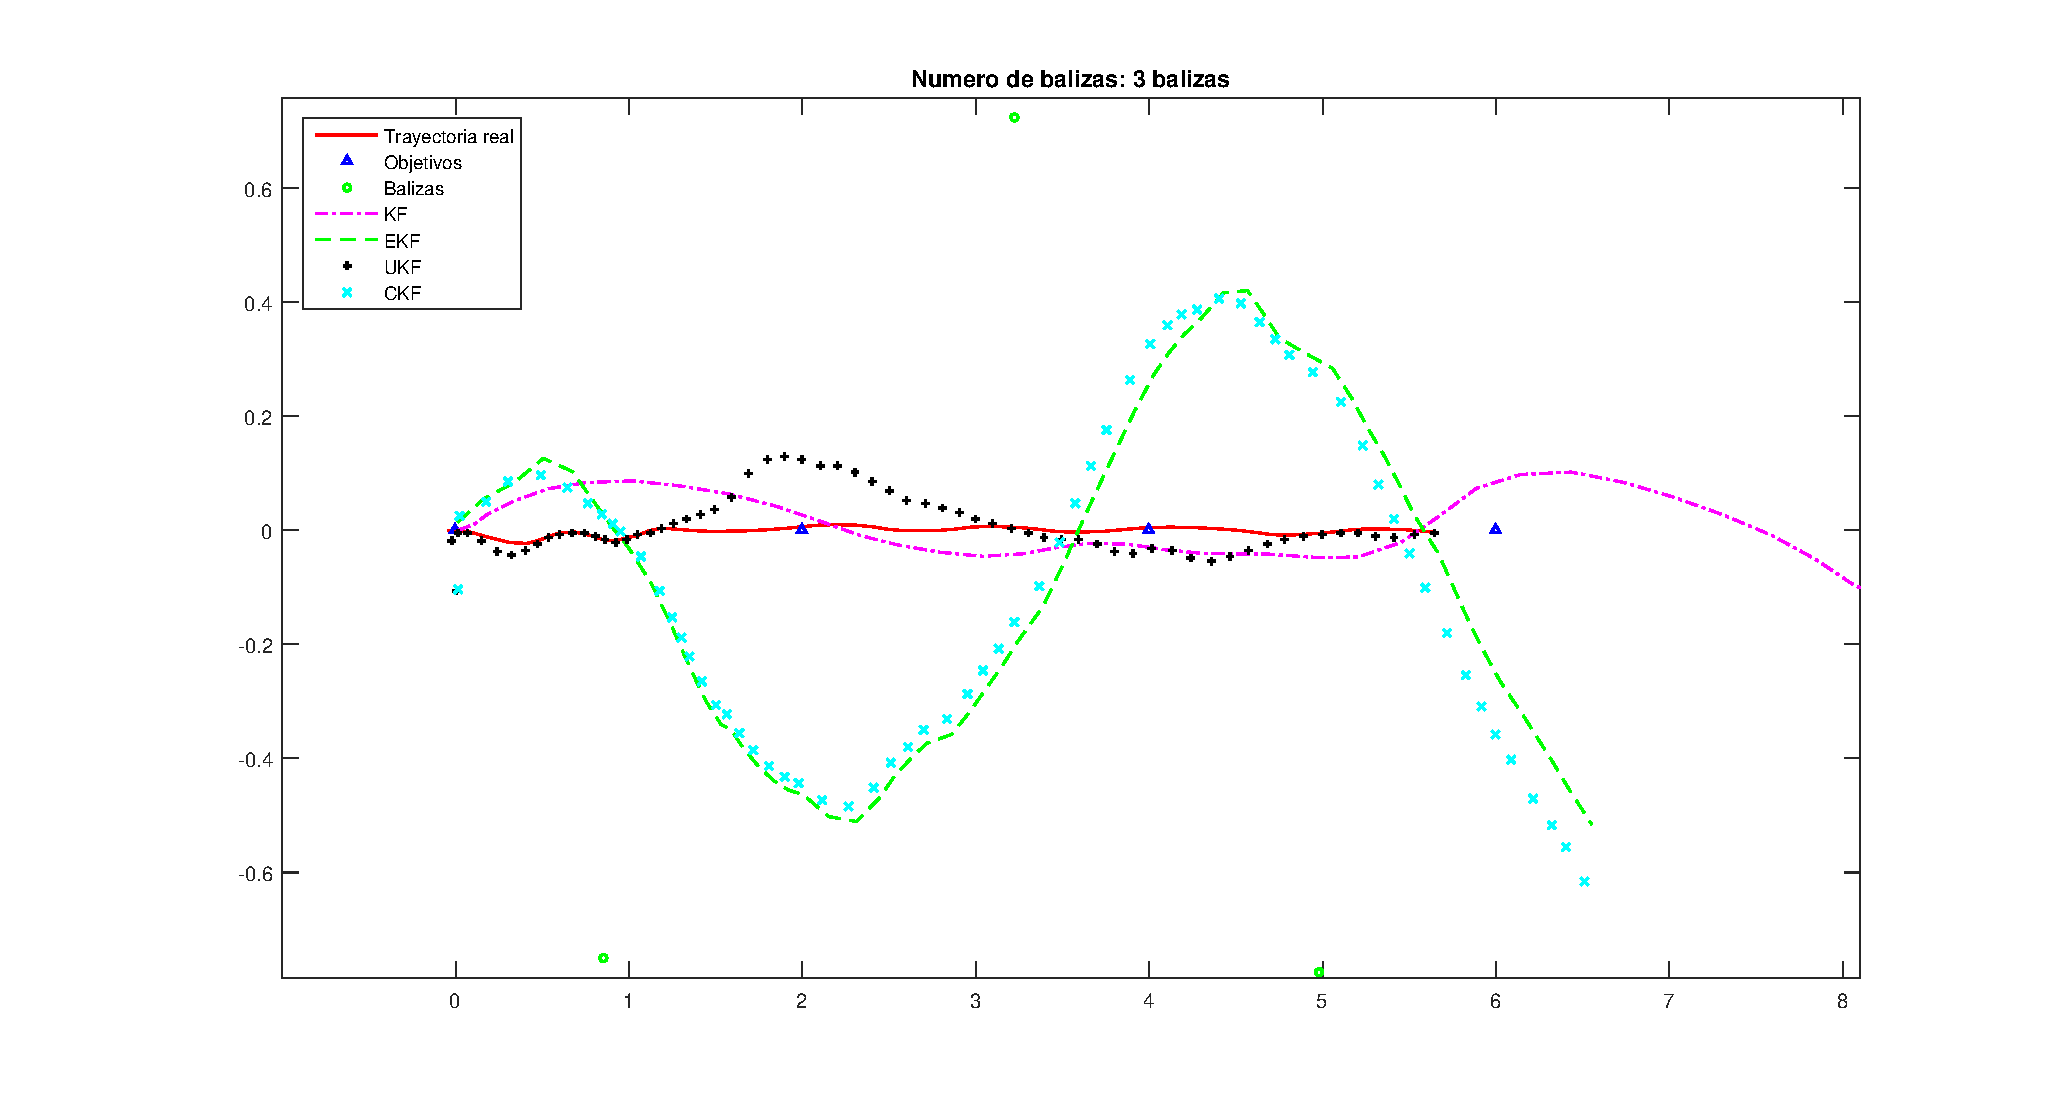
\includegraphics[scale=0.4]{Figura7}
\caption{Trayectoria recta 3 balizas} \label{Figura7}
\end{figure}
Vemos en la figura \ref{Grafico7} como el error disminuye a medida que aumentamos el número de balizas en la escena, lo cual es una de las premisas del filtro de Kalman , cuanta más información mejor estimación.
Además en la figura \ref{Figura7} podemos observar que cuando el \ac{EKF} y \ac{CKF} tienen poca información de las balizas, es decir tenemos pocas rodeando al robot, la estimación se vuelve totalmente errónea.
Por esta razón en la figura \ref{Figura7} vemos como se producen unas grandes oscilaciones en la estimación.
Hay que recordar que la trayectoria real mostrada en la figura difiere para cada una de las simulaciones de los filtros por lo que no hay que tomar esta como una referencia fiel de la realidad sino como una representación orientativa.

\subsection{Resultados para la trayectoria cuadrada}
Los resultados para esta serie de pruebas se muestran en las figuras .
\begin{figure}[ht!]
\centering
\includegraphics[scale=0.6]{Grafico8}
\caption{Experimento cuadrado variando número de balizas} \label{Grafico8}
\end{figure}
\begin{figure}[ht!]
\centering
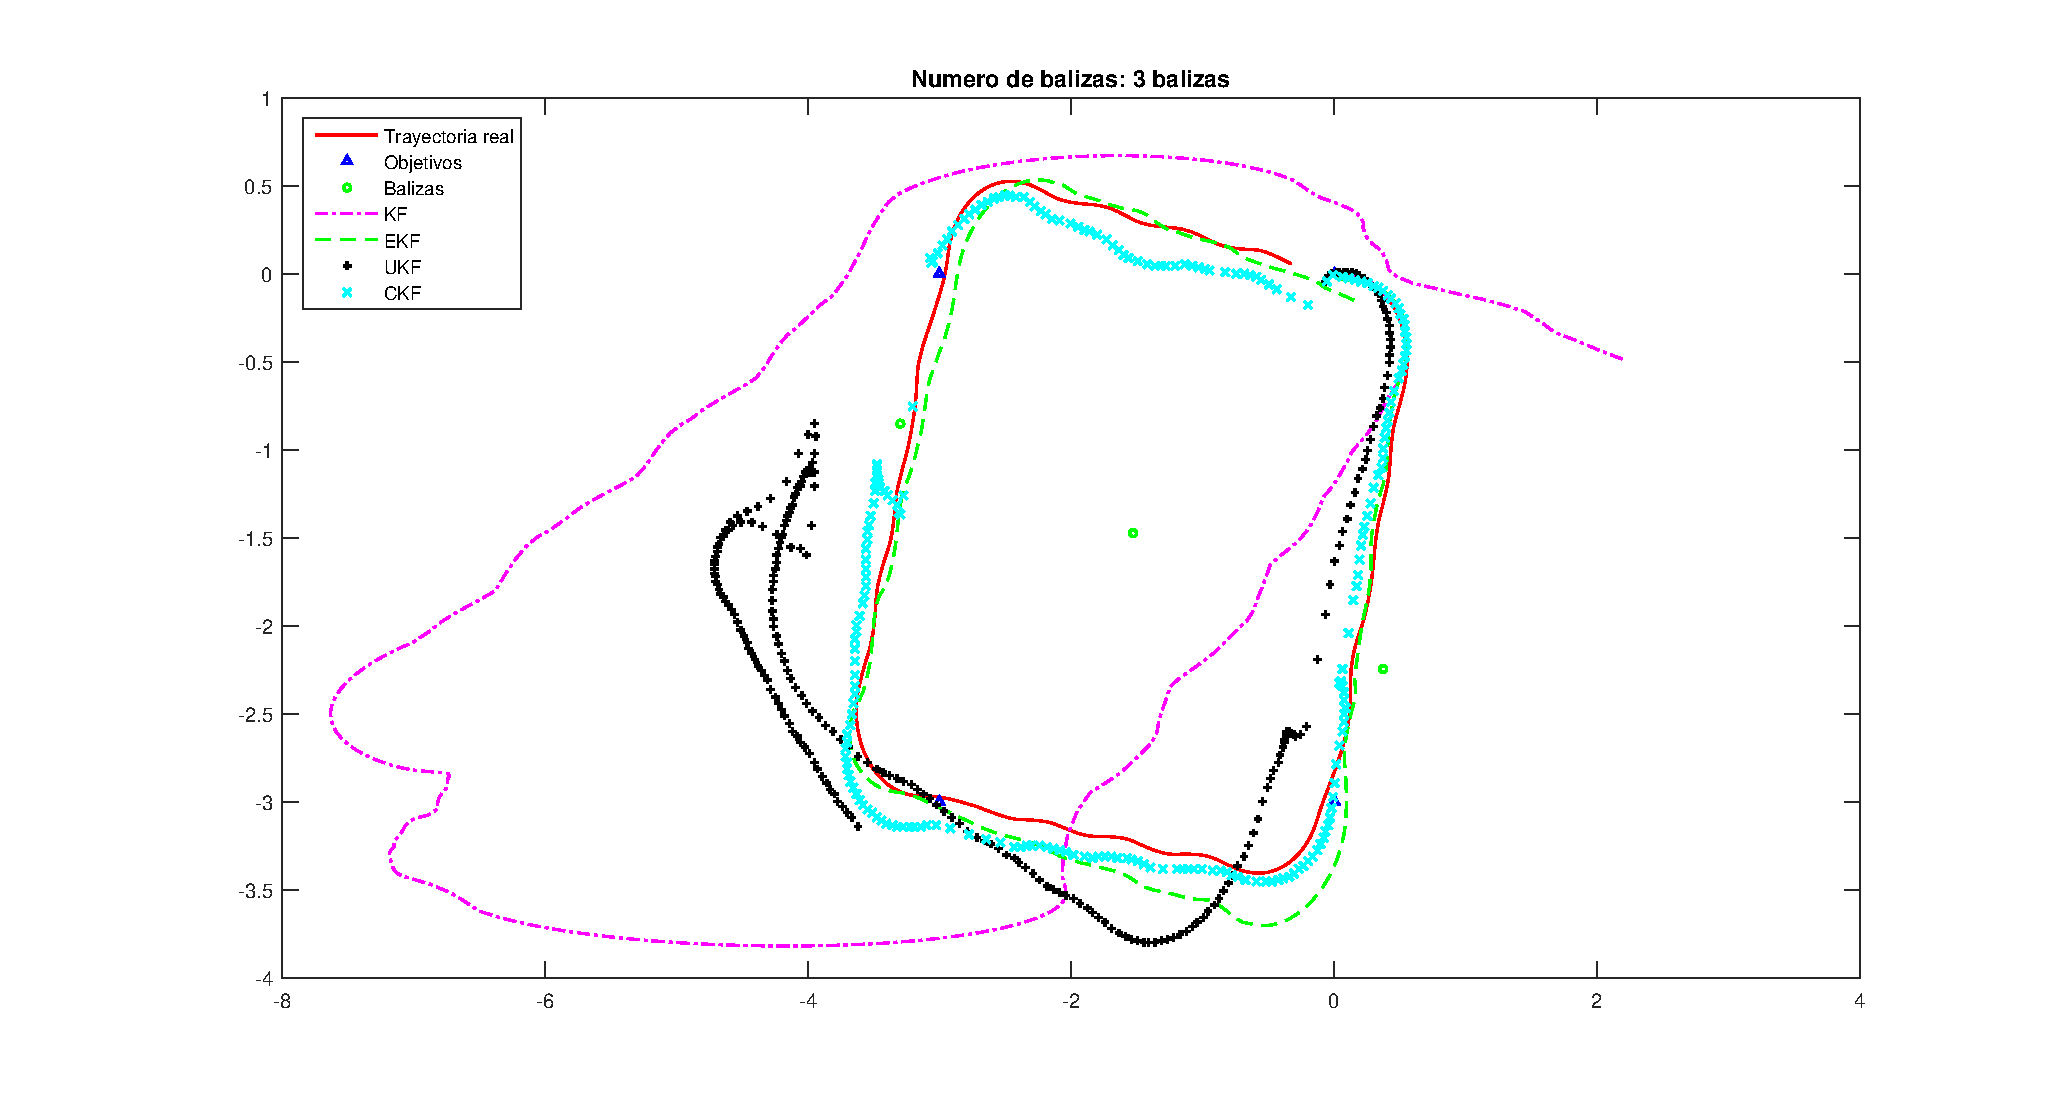
\includegraphics[scale=0.4]{Figura8}
\caption{Trayectoria cuadrada 3 balizas} \label{Figura8}
\end{figure}
Al igual que en el experimento anterior el error obtenido disminuye cuando aumentamos el número de balizas en la escena como vemos en la figura \ref{Grafico8}.
En este caso en la figura \ref{Figura8} podemos ver que el filtro de Kalman clásico presenta mucho error aunque este detalle no es relevante porque como ya hemos dicho la sintonización de este filtro no depende del número de balizas sino que depende únicamente de la odometría.
En esta figura, podemos ver como la estimación más acertada es la realizada por el \ac{CKF} y \ac{EKF} como también confirma la figura \ref{Grafico8}.

\subsection{Resultados para la trayectoria senoidal}
Los resultados de estas pruebas se muestran en las figuras \ref{Figura9} y \ref{Grafico9} .
\begin{figure}[ht!]
\centering
\includegraphics[scale=0.6]{Grafico9}
\caption{Experimento seno variando número de balizas} \label{Grafico9}
\end{figure}
\begin{figure}[ht!]
\centering
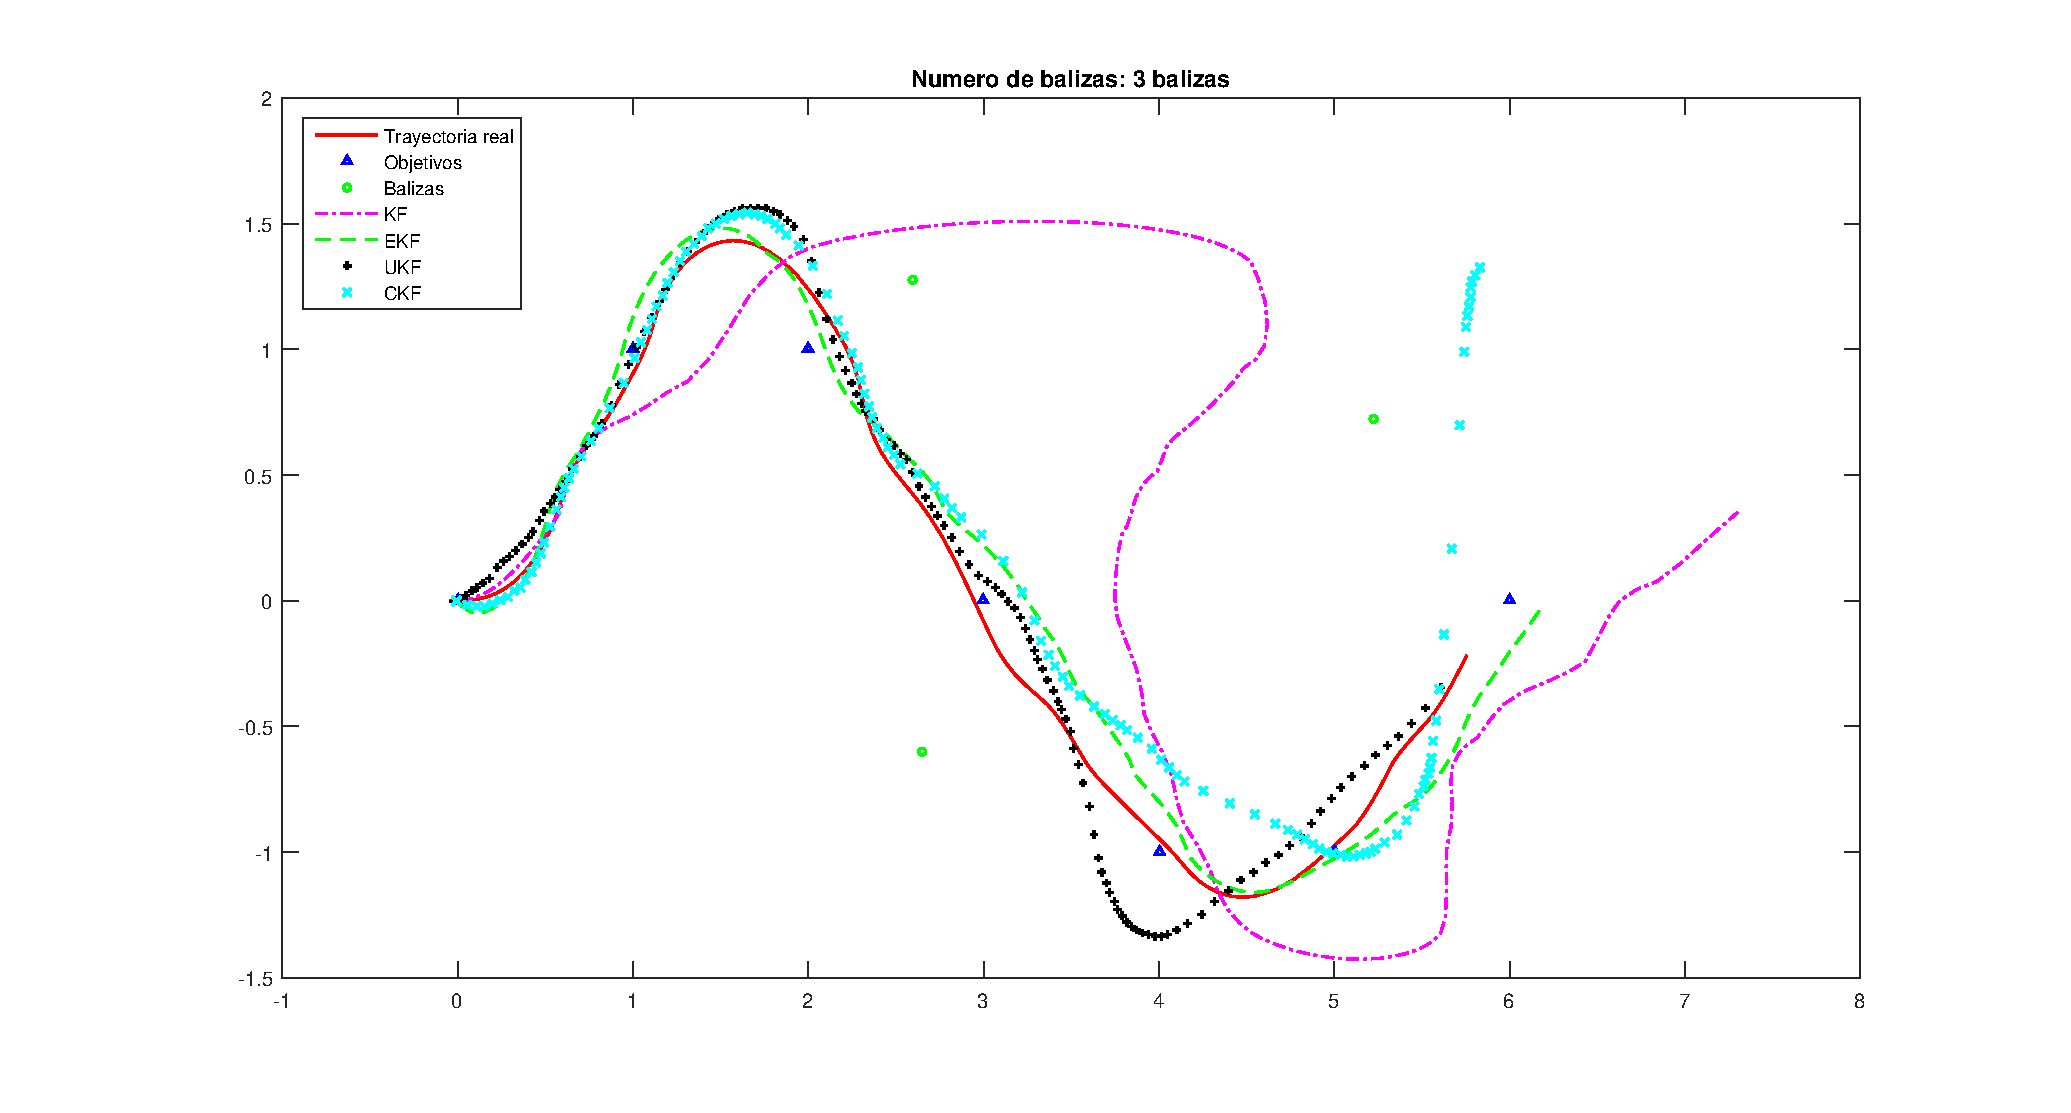
\includegraphics[scale=0.4]{Figura9}
\caption{Trayectoria senoidal 3 balizas} \label{Figura9}
\end{figure}
Para esta serie de experimentos el error entre filtros es bastante parecido.
Como vemos en la figura \ref{Grafico9} el error también disminuye a medida que aumentamos la información sensorial, lo que ha sido un punto en común entre todas las pruebas realizadas.
En la figura \ref{Figura9} podemos ver que las estimaciones de los filtros \ac{EKF}, \ac{UKF} y \ac{CKF} son muy parecidas entre sí.
También podemos observar este hecho en la figura \ref{Grafico9} donde vemos que los errores están próximos entre sí.

La conclusión para esta serie de experimentos es la siguiente : \textbf{El error en al estimación disminuye a medida que aumenta el número de balizas disponibles para tomar medidas. Los filtros por lo general se ven afectados en la misma medida por la falta de información sensorial. Si tuvieramos que destacar uno de ellos este sería el \ac{UKF} el cual tiende a aumentar mucho su error cuando la información sensorial es pobre por otra parte el \ac{CKF} es el que por lo general parece más robusto en cuanto a una disminución en la información sensorial.}
% * <amorellg@ull.edu.es> 2016-06-06T20:37:06.718Z:
%
% >  a la falta de información sensorial
%
% mejor: "a una disminución en la información sensorial"
%
% ^ <alu0100765755@ull.edu.es> 2016-06-07T09:47:48.130Z.

\section{Experimento 4: Rendimiento ante una trayectoria general}% * <amorellg@ull.edu.es> 2016-06-06T20:37:32.198Z:
%
% > Mejores condiciones de sintonización
%
% Rendimiento ante una trayectoria general
%
% ^ <alu0100765755@ull.edu.es> 2016-06-07T09:48:32.733Z.
En esta sección experimentaremos con la sintonización recomendada para los filtros para así  ver como se comporta cada uno en unas condiciones normalizadas de funcionamiento.
% * <amorellg@ull.edu.es> 2016-06-06T20:38:04.190Z:
%
% > a mejor sintonización
%
% sintonización recomendada
%
% ^ <alu0100765755@ull.edu.es> 2016-06-07T10:06:53.282Z.
Usaremos el modelo de medida de distancia para este experimento ya que es el más robusto.
Representaremos los resultados por medio de la tabla \ref{Exp_trayectoria_general} para ver cual ha sido el error para cada filtro además de mostrar en las figuras con  el resultado de la estimación para cada uno de los filtros utilizados.
Hay que tener en cuenta que las figuras seleccionadas son las que representan el peor caso en la estimación y lo realmente relevante son las medias obtenidas para los experimentos mostradas en la tabla \ref{Exp_trayectoria_general}.

\begin{table}[htbp]
\caption{Experimentos trayectoria general}
\begin{center}
\begin{tabular}{|l|c|c|l|c|c|c|c|}
\hline
\multicolumn{ 8}{|c|}{Experimento 4} \\ \hline
Recorrido & Deslizamiento & \multicolumn{ 2}{c|}{Ruido sensores (m)} & KF & EKF & UKF & CKF \\ \hline
Circuito  & 5,00\% & \multicolumn{ 2}{c|}{0,05} & 4.3& 1.4 & 1.355 &1.358 \\ \hline
\end{tabular}
\end{center}
\label{Exp_trayectoria_general}
\end{table}

\begin{figure}[ht!]
\centering
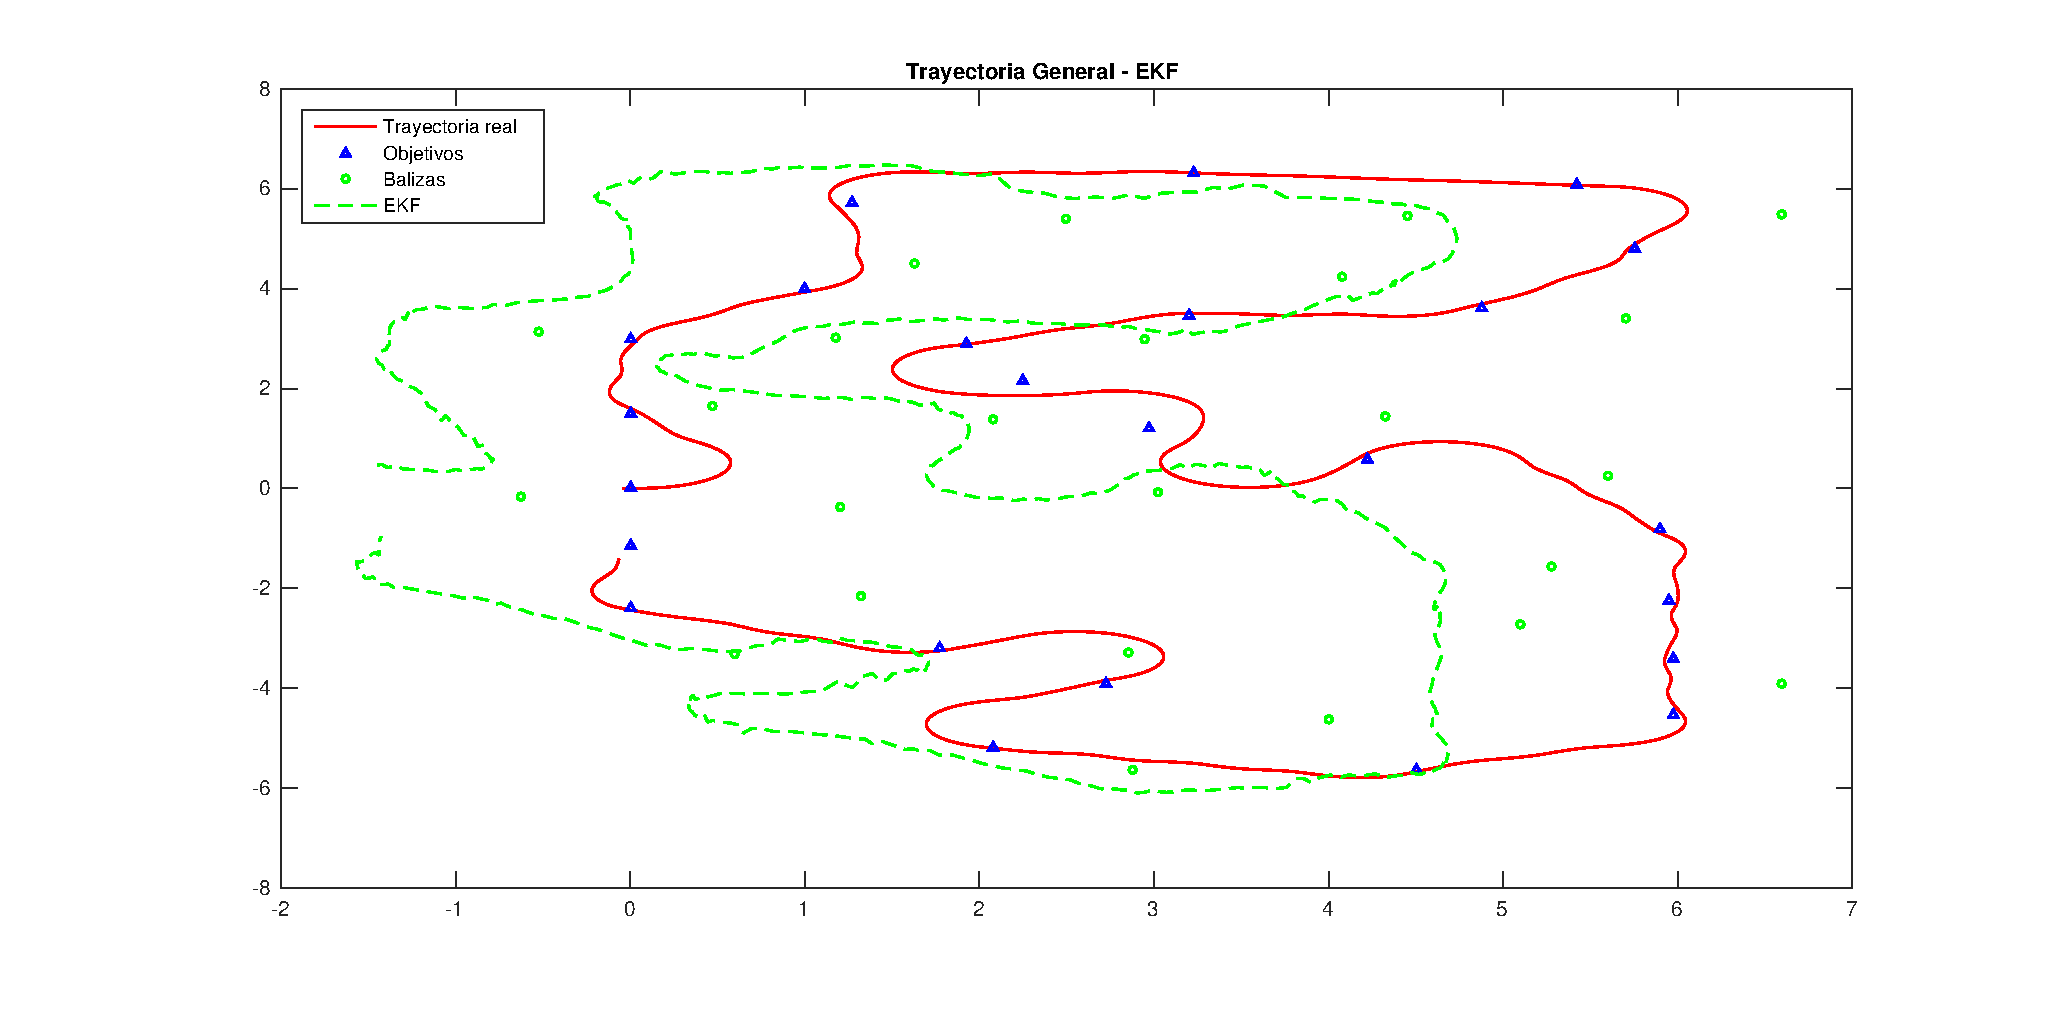
\includegraphics[scale=0.45]{Figura10_1}
\caption{Experimento trayectoria general EKF} \label{Figura10_1}
\end{figure}
\begin{figure}[ht!]
\centering
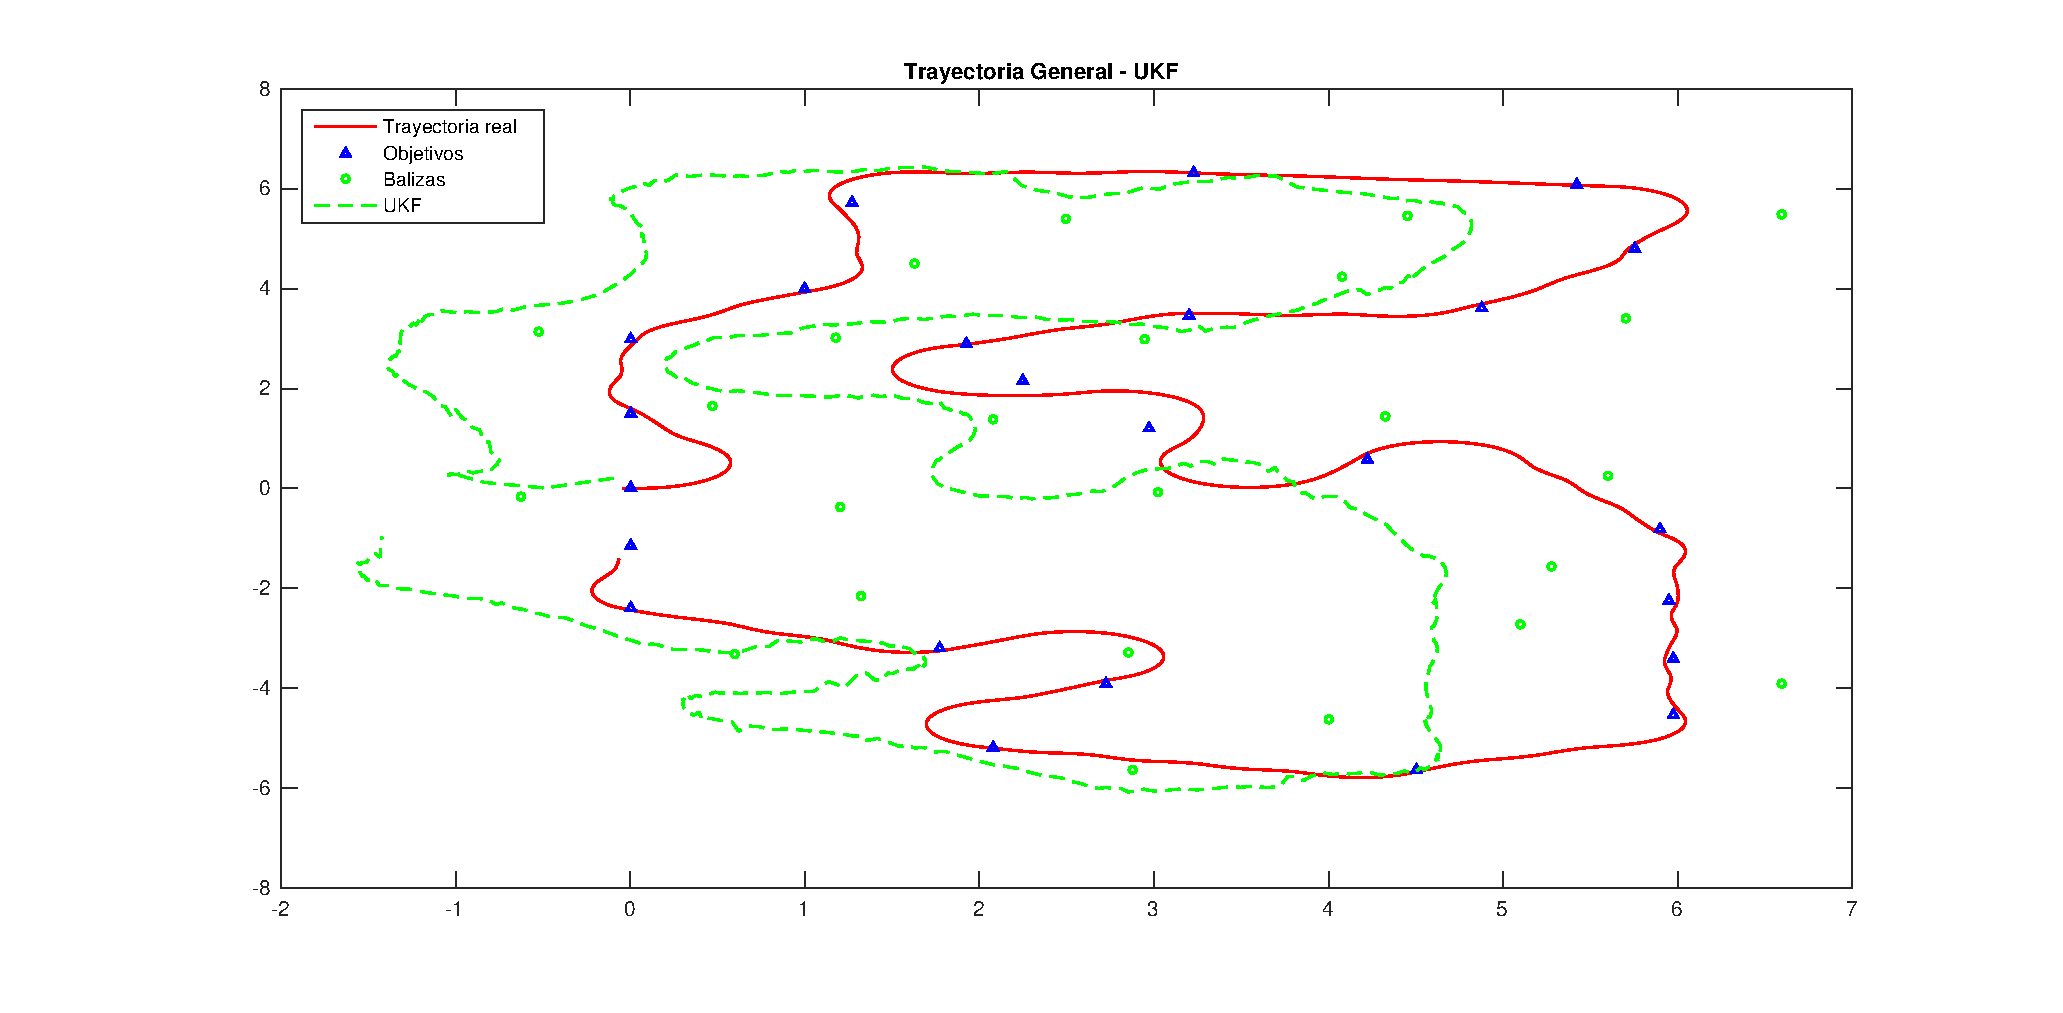
\includegraphics[scale=0.45]{Figura10_2}
\caption{Experimento trayectoria general UKF} \label{Figura10_2}
\end{figure}
\begin{figure}[ht!]
\centering
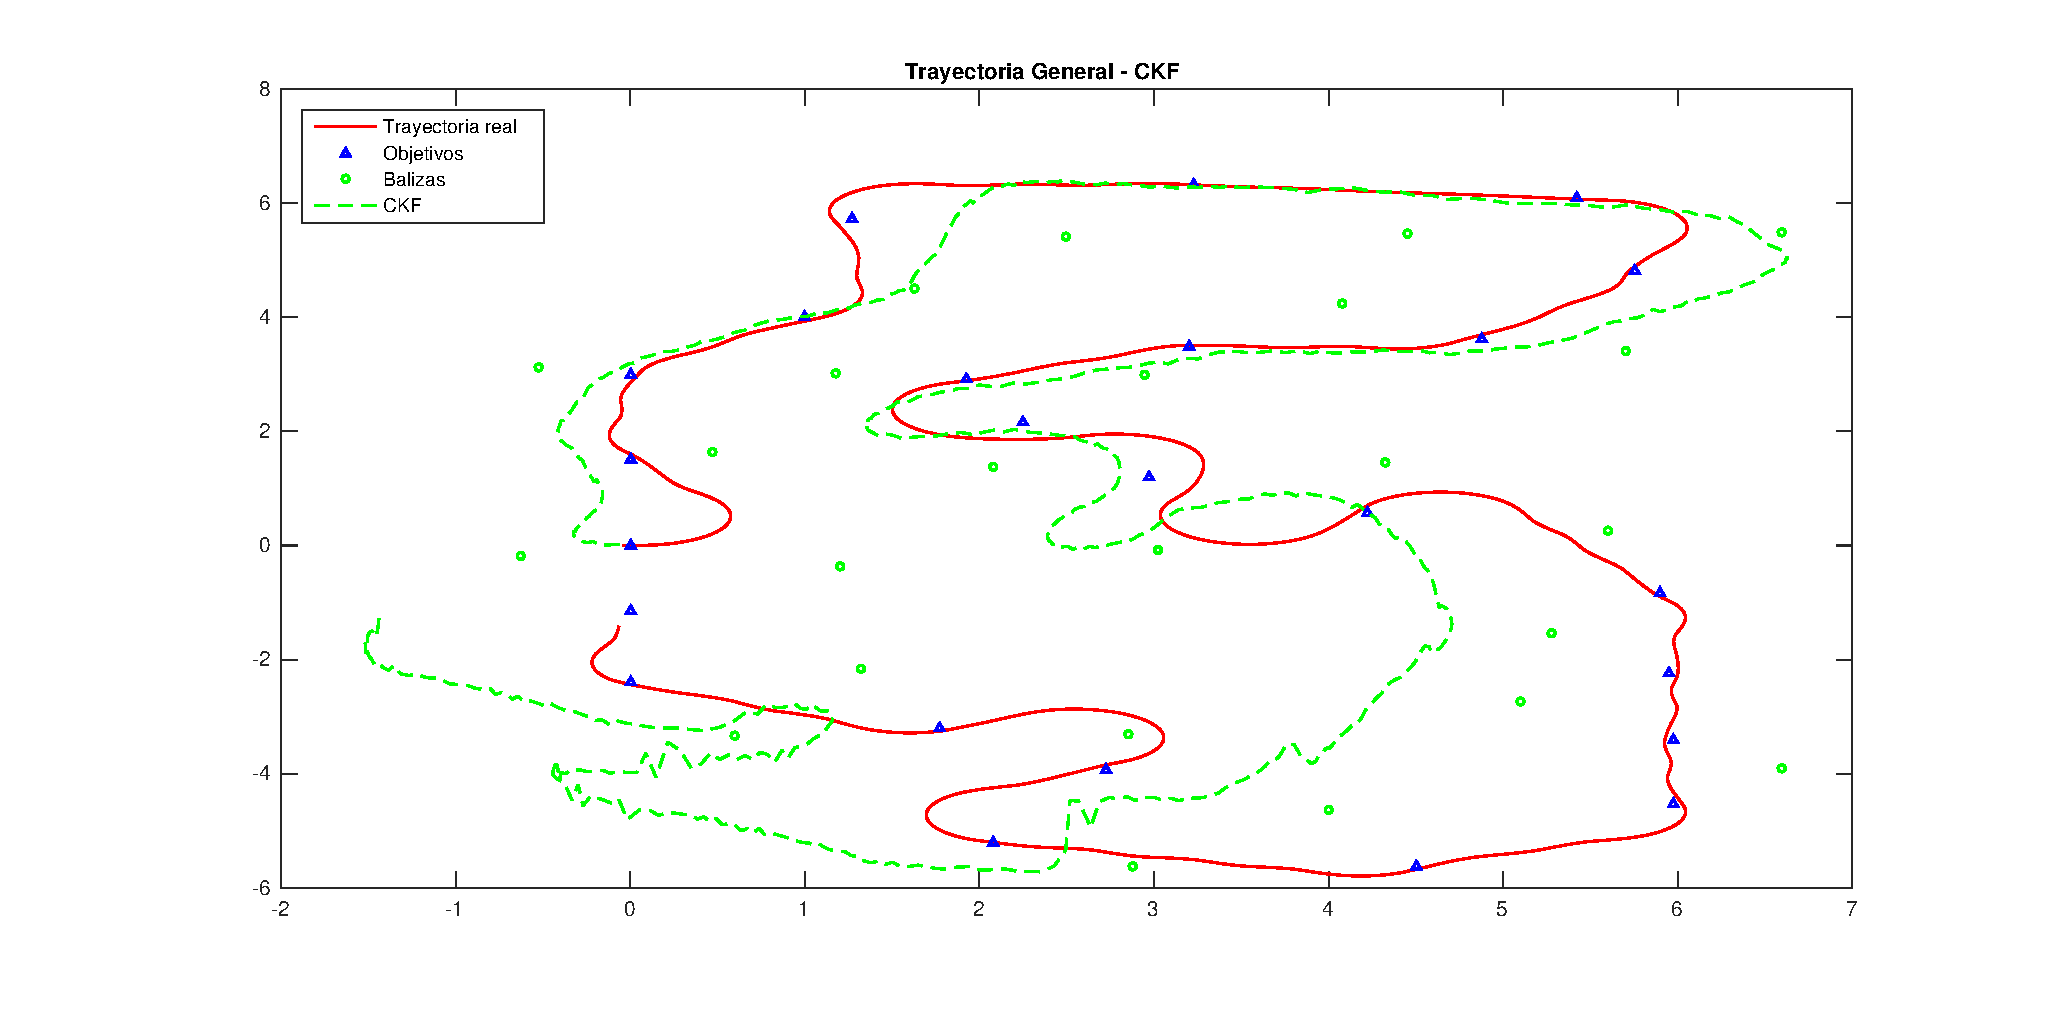
\includegraphics[scale=0.45]{Figura10_3}
\caption{Experimento trayectoria general CKF} \label{Figura10_3}
\end{figure}
 Podemos ver en la tabla \ref{Exp_trayectoria_general} que el filtro que ha obtenido el menor error en su estimación ha sido el \ac{UKF} seguido muy de cerca por el \ac{CKF}.
 En las figuras \ref{Figura10_1}, \ref{Figura10_2} y \ref{Figura10_3} podemos apreciar las diferencias entre las trayectorias debido al deslizamiento existente, ya que hace que la odometría de una información que hace imprecisa la estimación.
 Como vemos en la comparación de estas figuras, la estimación de los filtros es muy parecida, por lo que se ven afectados en la misma media por el deslizamiento.
% * <amorellg@ull.edu.es> 2016-06-06T20:53:58.958Z:
%
% > Es difícil llegar a saber cual es el mejor filtro en esta prueba ya que la colocación de las balizas, los deslizamientos y algunos otros factores pueden llegar a jugar un papel crucial.
%
% esto es lo que te comenté que habría que cambiar, en la conclusión general de este experimento sí se debería poder comparar  el error que  tiene cada filtro para la misma trayectoria
%
% ^ <alu0100765755@ull.edu.es> 2016-06-07T10:09:28.837Z.
 Podemos decir es que el \ac{UKF} ha sido el filtro que ha realizado la mejor estimación, aunque con muy poca diferencia sobre los demás como podemos ver en la tabla \ref{Exp_trayectoria_general} y la figura \ref{Figura10_2}.
 Por otra parte,como hemos dicho, en todos los filtros hemos implementado la odometría por lo que quizás de no haber implementado esta información sensorial la estimación podría haber cambiado.
 Aunque lo anterior fuera posible, el objetivo de esta prueba es testear los filtros en una situación en la que estén configurados de manera que incluyan la fusión sensorial.
 
La conclusión para esta serie de experimentos es la siguiente : \textbf{El \ac{UKF} ha sido el mejor adaptado a la trayectoria pero esto no quiere decir que sea el mejor filtro, como vemos los deslizamientos han generado que las trayectorias estimadas son bastante diferentes a las trayectorias reales debido a este motivo. Podemos concluir con este experimento que los deslizamientos pueden provocar muy malos resultados en la estimación  y aunque el \ac{UKF} muestre los mejores resultados el resto de filtros obtienen una estimación parecida. Sin embargo, el \ac{UKF} parece el que mejor se adapta a una trayectoria con deslizamientos. }

\section{Resultados generales}

Una vez hemos realizado todos los experimentos, tenemos que llegar a una conclusión global sobre todas la implementaciones que hemos hecho y sobre todo debemos sacar conclusiones acerca de los resultados obtenidos para las pruebas. 
Para facilitar la toma de decisiones hemos decidido dar una puntuación a la posición que ha obtenido cada filtro en la realización de los experimentos.
De esta manera estableceremos un ranking en el que posicionaremos cada uno de estos en orden y veremos como de cerca están unos de otros y además este nos permitirá tomar una decisión mucho más objetiva al respecto.
Las puntuaciones las hemos asignado en función de la posición obtenida en la realización del experimento, es decir, si por ejemplo el \ac{EKF} resulta hacer la mejor estimación en un experimento concreto se le sumarán 4 puntos, si es el segundo mejor se le sumarán 3 y así hasta llegar a 1 punto que corresponderá al filtro que quede en cuarto lugar.
Podemos ver en la tabla \ref{Tabla_puntuaciones} las puntuaciones obtenidas.
\begin{table}[htbp]
\caption{Puntuaciones obtenidas por los filtros}
\begin{center}
\begin{tabular}{|c|c|c|c|c|}
\hline
Experimento & \textbf{KF} & \textbf{EKF} & \textbf{UKF} & \textbf{CKF} \\ \hline
1 & 1 & 2 & 4 & 3 \\ \hline
2 & 1 & 2 & 3 & 4 \\ \hline
3 & 1 & 2 & 4 & 3 \\ \hline
4 & 1 & 4 & 2 & 3 \\ \hline
5 & 1 & 2 & 4 & 3 \\ \hline
6 & 1 & 2 & 4 & 3 \\ \hline
7 & 1 & 3 & 2 & 4 \\ \hline
8 & 1 & 2 & 4 & 3 \\ \hline
9 & 1 & 3 & 2 & 4 \\ \hline
10 & 1 & 4 & 2 & 3 \\ \hline
11 & 1 & 3 & 2 & 4 \\ \hline
12 & 1 & 3 & 2 & 4 \\ \hline
13 & 1 & 2 & 4 & 3 \\ \hline
14 & 1 & 4 & 2 & 3 \\ \hline
15 & 1 & 3 & 2 & 4 \\ \hline
16 & 1 & 2 & 4 & 3 \\ \hline
\textbf{TOTAL} & \textbf{\textit{16}} & \textbf{\textit{43}} & \textbf{\textit{47}} & \textbf{\textit{54}} \\ \hline
\end{tabular}
\end{center}
\label{Tabla_puntuaciones}
\end{table}



Como podemos observar el filtro que ha resultado tener el mejor desempeño general en todas la pruebas realizadas ha sido el \ac{CKF} lo cual no es una sorpresa si pensamos que este filtro es una de las últimas modificaciones ideadas para el filtro de Kalman clásico y por lo tanto su funcionamiento se supone más óptimo.
En segundo lugar tenemos al \ac{UKF}, este ha quedado en esta posición debido muy probablemente a su poca robustez a la hora de trabajar con distintas funciones de medida y con poca información sensorial lo cual provoca que realice malas estimaciones.
Por otro lado el \ac{UKF} suele mostrarse muy robusto cuando trabaja con trayectorias en las que se sufren deslizamientos.
Al \ac{UKF} lo sigue  el \ac{EKF} que en casi todos los experimentos se ha mantenido en la mitad de la clasificación, no es un filtro que haya destacado en nada positivamente pero tampoco lo ha hecho de manera negativa.
En último lugar se encuentra el \ac{KF} que como era de esperar sería el filtro que presentaría los peores resultados de los cuatro estudiados.
Sin embargo, en las implementaciones que hemos realizado sobre el \ac{KF} hemos visto que aunque su estimación es peor que en el caso de los otros tres filtros esta no suele cometer errores demasiado acusados cuando el deslizamiento es bajo.
Por contra, como vimos en el experimento de la trayectoria completa, si el deslizamiento es grande la estimación del \ac{KF} es totalmente errónea, comentiendo así un error inevitable para esta implementación del filtro.
